\begin{savequote}[8cm]
Two MCs can't occupy the same space at the same time,
it's against the laws of physics.
\qauthor{--- Lauryn Hill, \textit{Zealots}}
\end{savequote}

\chapter{\label{ch:3-methods}Theory and methodology}

\minitoc

%% Books:

% For a really nice explanation of solid state QM basics - bloch waves, an electron in a crystal potential etc, see Lundstrom "fundamentals of carrier transport"

\section{Introduction} 

In this chapter I present the theory and methodology that underlies the work in this thesis. The chapter starts with an introduction to quantum chemistry and Density Functional Theory (DFT); first I introduce the theoretical concepts, then I provide some details about how DFT is implemented in practice. Later in the chapter I outline how we can use DFT energies combined with a series of post-processing steps to predict defect formation energies and charge transition levels. The chapter ends with an introduction to the theory of lattice dynamics and how this theory is used to calculate the vibrational properties of a material. 

\section{Quantum chemistry}

\subsection{The Schr\"{o}dinger equation}

A fundamental postulate of quantum mechanics is that for any physical system there is an associated wavefunction that contains all of the system information.
The Schr\"{o}dinger equation describes the wavefunction of a quantum mechanical system.  Once the Schr\"{o}dinger equation is solved, and a wavefunction is found, all the physical properties of that system follow. 
The general form of the many-body Schr\"{o}dinger equation is:\autocite{Kaxiras2007}
\begin{equation}
\hat{H}\Psi(\{\textbf{R}_I;\textbf{r}_i\}) = E\Psi(\{\textbf{R}_I;\textbf{r}_i\}),
\end{equation}
where $\Psi(\{\textbf{R}_I;\textbf{r}_i\})$ is the many-body wavefunction that describes the state of the system with ions in positions $\{\textbf{R}_I\}$ and electrons described by the variables $\{\textbf{r}_i\}$.
The Hamiltonian $\hat{H}$ is an operator corresponding to the sum of the kinetic and potential energies for all particles in a system. 

To take a simple example system, the time-independent non-relativistic Hamiltonian for a single hydrogen atom is:
\begin{equation} \label{singleparticle}
\hat{H} = -\frac{\hbar^2}{2M_1}\nabla_{\textbf{R}_1}^2-\frac{\hbar^2}{2m_e}\nabla_{\textbf{r}_1}^2-\frac{e^2}{\lvert\textbf{R}_1-\textbf{r}_1\rvert},
\end{equation}
where the first term is the kinetic energy of the hydrogen ion with mass $M_1$ and the second term is the kinetic energy of the electron with mass $m_e$. The third term is the Coulomb potential energy due to the interaction between the ion at position $R_1$ and electron at position $r_1$. 

For systems with multiple ions and electrons, the Hamiltonian is given by:\autocite{Kaxiras2007}
\begin{equation} \label{manybodyH}
\hat{H} = -\sum_{I}\frac{\hbar^2}{2M_I}\nabla_{\textbf{R}_I}^2-\sum_{i}\frac{\hbar^2}{2m_e}\nabla_{\textbf{r}_i}^2 +\sum_{i<j}\frac{e^2}{\lvert\textbf{r}_i-\textbf{r}_j\rvert}-\sum_{i}\sum_{I}\frac{Z_Ie^2}{\lvert\textbf{R}_I-\textbf{r}_i\rvert}+\sum_{I<J}\frac{Z_IZ_Je^2}{\lvert\textbf{R}_i-\textbf{R}_j\rvert}.
\end{equation}
The first two terms correspond to the kinetic energy of the ions and electrons, respectively. The third term describes the repulsive electrostatic interactions between two electrons with charge $e$ and the fifth term describes the repulsive interactions between ions of charge $Z_Ie$ and $Z_Je$. The fourth term describes the attractive electrostatic interactions between an electron and positively charged ion with charge $Z_I$. The following expression will be used to simplify the latter term:
\begin{equation}
v_\textrm{ext}(\textbf{r}) = -\sum_I\frac{Z_Ie^2}{\lvert\textbf{R}_I-\textbf{r}\rvert},
\end{equation}
where $v_\textrm{ext}$ is the external potential felt by a single electron. 

The Born-Oppenheimer approximation can be used to simplify Equation \ref{manybodyH}.\autocite{Born1927} This approximation assumes that, because the ions are significantly heavier than the electrons, the ions are moving slowly in space and the electrons can respond instantaneously to any ionic motion. The ions are treated as fixed points and the ion kinetic energy term in Equation \ref{manybodyH} is zero. Only the electronic sub-system is treated quantum mechanically and so we can neglect the ion-ion term in Equation \ref{manybodyH} as it is independent of the electronic degrees of freedom.
Under the Born-Oppenheimer approximation the many-body Hamiltonian becomes:\autocite{Kaxiras2007}
\begin{equation}
\hat{H} = -\sum_{i}\frac{\hbar^2}{2m_e}\nabla_{\textbf{r}_i}^2 +\sum_{i<j}\frac{e^2}{\lvert\textbf{r}_i-\textbf{r}_j\rvert}+\sum_{i}v_\textrm{ext}(\textbf{r}_i).
\end{equation}



\subsection{The Hartree and Hartree-Fock approximations}

For a simple system, such as the particle in a box system or hydrogen atom, the Schr\"{o}dinger equation can be solved exactly. Unfortunately it is not possible to solve the Schr\"{o}dinger equation exactly for more complex systems, where there are multiple electrons interacting with each other (N-body or many-body systems). 
Hartree-Fock methods and Kohn-Sham DFT provide ways to obtain an approximate solution to the Schr\"{o}dinger equation for systems of interest. They do this by mapping the interacting problem onto a non-interacting problem with an effective potential. In doing so, the dimensionality of the problem is greatly reduced. Instead of solving one N-dimensional computationally intractable problem, N one-dimensional problems are solved (Figure \ref{decouple}). These methods provide a compromise between accuracy and computational efficiency.

\begin{figure}[h]
\centering
  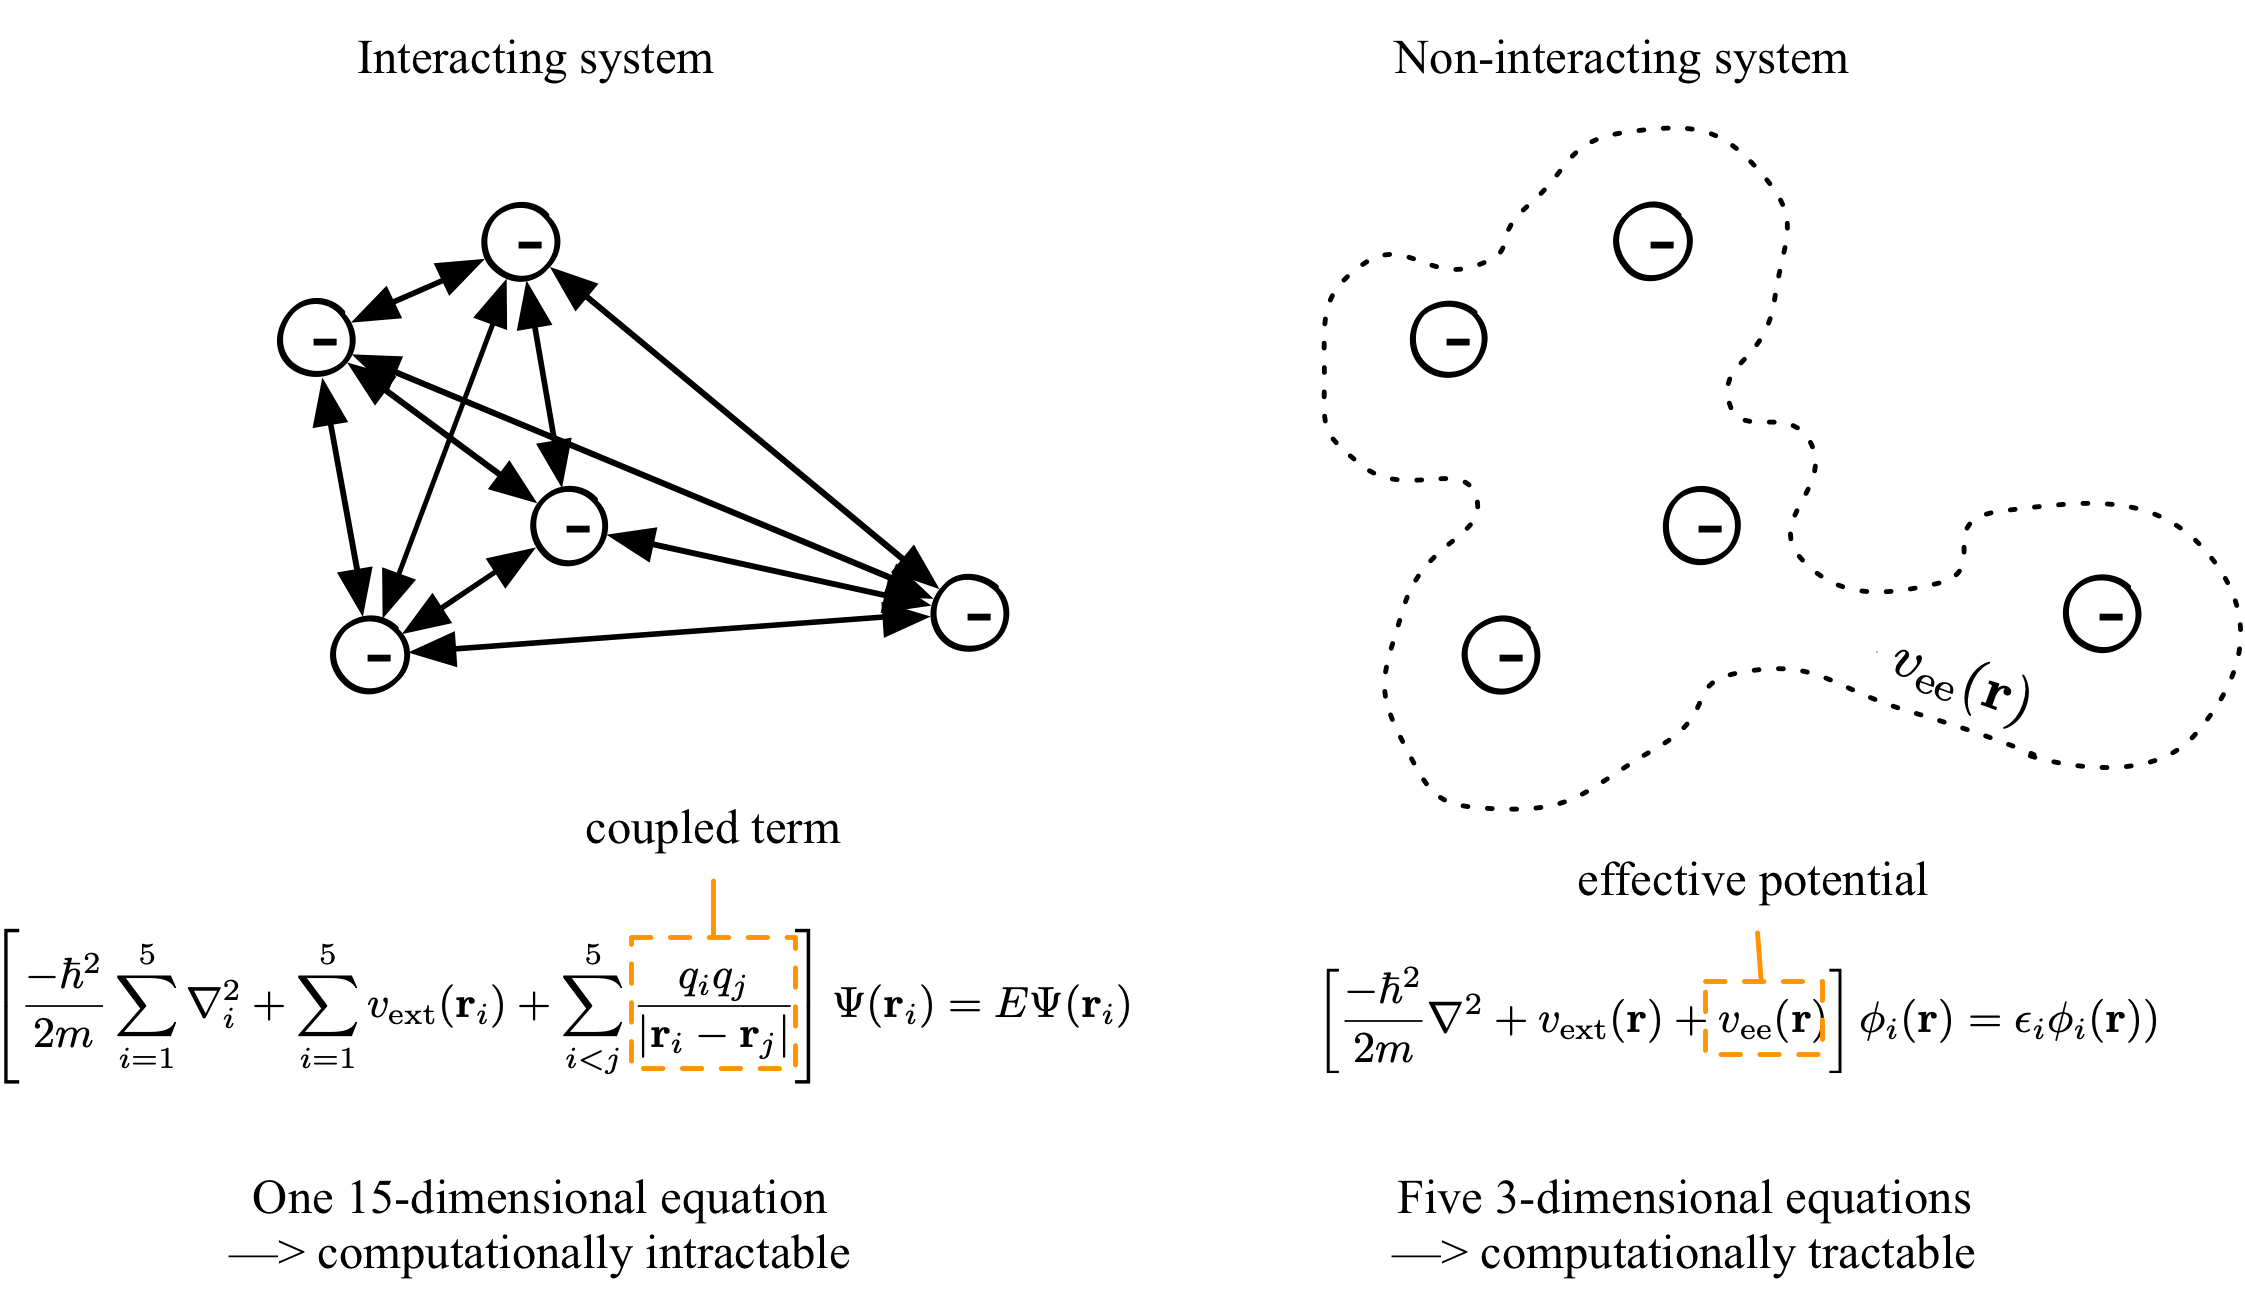
\includegraphics[width=1.0\columnwidth]{figures/ch3/decouple.png}
  \caption[Interacting and non-interacting particle systems]{Schematic outlining the equivalence between a system of interacting particles and a system of non-interacting particles in an effective potential $v_{ee}$. The underlying idea is that an interaction can be replaced by the equivalent potential. This maps the interacting 3N-dimensional problem onto N 3-dimensional problems. For the non-interacting case $\phi_i$ is used to denote a single particle wavefunction. $v_{\textrm{ext}}$ describes the interaction between an electron and the surrounding ions.} %update so q1q2 in couple term in picture
  \label{decouple}
\end{figure}  %%% NEED TO ADJUST FIGURE

The Hartree approximation assumes that the many-body wavefunction $\Psi^{\textrm{H}}(\{\textbf{r}_i\})$ is simply a product of independent single electron states $\phi_i(\textbf{r}_i)$:\autocite{Hartree1928}
\begin{equation}
\Psi^{\textrm{H}}(\{\textbf{r}_i\}) = \phi_1(\textbf{r}_1)\phi_2(\textbf{r}_2)\ldots\phi_n(\textbf{r}_n).
\end{equation}

As each state is independent, the system Hamiltonian $\hat{H}$ becomes the sum over the Hamiltonian for each single electron state $\hat{h}_i$:
\begin{equation}
\hat{H} = \sum_i\hat{h}_i,
\end{equation}

Under the Hartree approximation, $\hat{h}_i$ is given by:
\begin{align}
\hat{h}_i &= -\frac{\hbar^2}{2m_e}\nabla_{\textbf{r}}^2 + v_\mathrm{ext}(\textbf{r}) + v_i^\textrm{H}(\textbf{r}) \\
v_i^\textrm{H}(\textbf{r}) &= e^2\sum_{j\neq i} \int\frac{\rho_j(\textbf{r}')}{\lvert\textbf{r}-\textbf{r}'\rvert}\textrm{d}\textbf{r}' \\ \label{singleparticledensity}
\rho_j &= \lvert\phi_j\rvert^2.
\end{align}

The $v_i^\textrm{H}(\textbf{r})$ term corresponds to the average electrostatic repulsion between electrons and is called the Hartree potential. A self-consistent field method (discussed further in Section \ref{SCFsubsection}) is needed to solve the time-independent Schr\"{o}dinger equation $\hat{h}_i\phi_i=\epsilon_i\phi_i$ for $\phi_i$, as the Hartree potential depends on the charge density $\rho_j$, which itself depends on the single-particle wavefunction $\phi_j$. 

% INCLUDE HERE THE SELF INTERACTION ERROR?
%Hartree-Fock (HF) methods introduce the concept of fictitious non-interacting one-electron orbitals $\phi$ as a way of solving the Schr\"{o}dinger equation. The one-electron orbitals are combined using a Slater determinant to produce the HF many-body wavefunction.\autocite{Burke2007} 

The Pauli Exclusion Principle states that the many-body wavefunction of an electron (or any particle with a half-integer spin quantum number) must be antisymmetric with respect to exchange - i.e. the wavefunction must change sign if any two electrons are exchanged.\autocite{Kaxiras2007} The Hartree many-body wavefunction $\Psi^{\textrm{H}}$ does not obey this rule. However the single electron states $\phi_i$ can be combined to form a Slater determinant,\autocite{Slater1929} which is antisymmetrical with respect to exchange:
\begin{equation} \label{slaterdet}
\Psi^{\textrm{HF}}(\{\textbf{r}_i\}) = \frac{1}{\sqrt{N!}}
\begin{vmatrix}
\phi_1(\textbf{r}_1)&\phi_1(\textbf{r}_2)&\ldots&\phi_1(\textbf{r}_n) \\
\phi_2(\textbf{r}_1)&\phi_2(\textbf{r}_2)&\ldots&\phi_2(\textbf{r}_n) \\
\cdot & \cdot & & \cdot \\
\cdot & \cdot & & \cdot \\
\cdot & \cdot & & \cdot \\
\phi_n(\textbf{r}_1)&\phi_n(\textbf{r}_2)&\ldots&\phi_n(\textbf{r}_n) \\
\end{vmatrix}.
\end{equation}

Forming a many-body wavefunction $\Psi^{\textrm{HF}}(\{\textbf{r}_i\})$ from the Slater determinant of single particle states is the Hartree-Fock approximation. To solve the Schr\"{o}dinger equation and find the ground state (lowest energy) solution for $\Psi^{\textrm{HF}}$ a variational method can be used.\autocite{Fock1930} In addition, the energy of each single particle state $\epsilon_i$ is minimised with respect to $\phi_i$, and $\{\phi_i\}$ form an orthonormal basis. Applying these principles results in the Hartree-Fock equations:\autocite{Fock1930}
\begin{align}
\bigg[-\frac{\hbar^2}{2m_i}\nabla_{\textbf{r}}^2  + v_\mathrm{ext}(\textbf{r}) &+ v_i^\textrm{H}\bigg]\phi_i(\mathbf{r})-v_i^\textrm{X}(\mathbf{r})\phi_j(\mathbf{r}) = \epsilon_i\phi_i(\mathbf{r}), \\
v_i^\textrm{X}(\mathbf{r}) &= e^2\sum_{j\neq i}\int \frac{\phi_j^*(\mathbf{r}')\phi_i(\mathbf{r}')}{\lvert\mathbf{r}-\mathbf{r}'\rvert}\textrm{d}\mathbf{r}'.
\end{align}
% http://nucleartalent.github.io/Course2ManyBodyMethods/doc/pub/hfock/html/hfock-bs.html

$v_i^\textrm{X}$ accounts for the spin exchange interaction between electrons, whereby two identical electrons (i.e. electrons with the same spin and momentum) cannot occupy the same space at the same time. This results in a repulsion between electrons with parallel spins.
%IT CANCELS ERROR FROM THE SELF INTERACTION OF THE HARTREE TERM

Hartree-Fock methods build upon the classical mean-field approach of the Hartree approximation to include the quantum spin nature of electrons.
However the Hartree-Fock approximation does not give an exact solution to the Schr\"{o}dinger equation as the true many body wavefunction is not formed from a simple Slater determinant. As a result, electron correlation -- the correlated motion of electrons with anti-parallel spins as a result of their mutual coulombic repulsion -- is ignored.
% from http://newton.ex.ac.uk/research/qsystems/people/coomer/dft_intro.html



\section{Density Functional Theory: basic concepts} \label{DFTtheory}

Density Functional Theory (DFT) is the most commonly used electronic structure method in condensed matter physics and quantum chemistry. The principle underlying DFT is that any ground state property of an interacting system can be determined by the electron density of a non-interacting system. We avoid specifying the form of the many-body wavefunction all together and no longer need to start with an approximation to the many-body wavefunction, as in the Hartree-Fock approach. Instead, the many-body effects of electron exchange and correlation are included as a functional of electron density.

DFT can be used to predict material properties including electron density, total energy, equilibrium structure, vibrational frequencies, and properties relating to differences in total energy, such as defect formation energy or surface energy. 
As DFT is a ground state theory we are not able to calculate properties relating to excited states and, without further calculations such as those outlined in Section \ref{sec:latticedynamics}, results do not incorporate the effects of temperature. 

The theoretical basis for DFT was established in 1964 through the work of Walter Kohn and Pierre Hohenberg.\autocite{Hohenberg1964} This was further developed by Walter Kohn and Lu Jeu Sham to produce Kohn-Sham DFT.\autocite{Kohn1965} However it was not until the late 1980's that approximations to the exchange-correlation functional were built so that DFT could be used in practice. 

There are a growing number of codes that implement DFT. 
Although some codes aspire to a blackbox approach, with the user protected from the underlying mechanics of DFT, for most systems of interest an understanding of the underlying approximations and parameters used are required for reliable results.

Finally, a note on the name. A function accepts one or more numbers as input and produces a number as output. Likewise, a functional accepts one or more \textit{functions} as inputs, and produces a number as output. In DFT the functional is the electron density which is itself a function of space and time.

\subsection{The Hohenberg-Kohn theorems}

The 1964 Hohenberg-Kohn paper\autocite{Hohenberg1964} contains two key results: (i) the ground state electron density uniquely determines the ground state electronic wave function and, following this, all properties of the system; (ii) the true density functional for the electronic energy assumes its minimum for the correct ground-state density.\autocite{Scuseria05}

The potentials -- external ($v_\mathrm{ext}$), coulomb ($v_i^H$) and exchange ($v_i^X$) -- in Hartree-Fock methods determine the properties of a system. Hohenberg and Kohn demonstrated that the electron density $\rho$ can be used to uniquely characterise the system and rather than solving the Schr\"{o}dinger equation for the wavefunction, we can solve it for the electron density.

First, Hohenberg and Kohn proved that the electron density is uniquely defined for a given external potential (electron-ion interaction). Their proof uses \textit{reductio ad adsurdum}; they first assume that two different external potentials can lead to the same density, and then show that this assumption leads to an impossible contradiction.\autocite{Burke2007} 
Second, we know that as the external potential is the only thing that differs from system to system, it is this which uniquely determines the system wavefunction. It follows that the electron density $\rho(\textbf{r})$ uniquely determines the system wavefunction and all derived properties, including the total energy $E$ of the system:\autocite{Kaxiras2007}
\begin{align}
E\left[\rho(\textbf{r})\right]&=\int v_{\textrm{ext}}(\textbf{r})\rho(\textbf{r})d\textbf{r}+T\left[\rho(\textbf{r})\right]+J\left[\rho(\textbf{r})\right]+E_{\textrm{xc}}\left[\rho(\textbf{r})\right] \\
&=\int v_{\textrm{ext}}(\textbf{r})\rho(\textbf{r})d\textbf{r}+F\left[\rho(\textbf{r})\right],   
\end{align}
where $T\left[\rho\right]$, $J\left[\rho\right]$ and $E_\textrm{xc}\left[\rho\right]$ describe the kinetic, classical electrostatic and exchange-correlation energies respectively. 
For a fixed number of electrons the functional $F\left[\rho(\textbf{r})\right]$ is universal, and the only thing that varies between systems is the external potential. The problem is that the exact form of this functional is unknown.

In addition to the above, Hohenberg and Kohn demonstrated that the energy functional $E\left[\rho(\textbf{r})\right]$ is minimised for the correct ground state density corresponding to $v_\mathrm{ext}(\textbf{r})$.\autocite{Hohenberg1964}

\subsection{The Kohn-Sham formalism} \label{KSformalismsubsection}

The Kohn-Sham (KS) formalism provides a practical way to apply the Hohenberg-Kohn theorem. The KS theorem shows that for any \textit{interacting} system with ground state density $\rho(\textbf{\textrm{r}})$ there exists a \textit{non-interacting} system with the same ground-state $\rho(\textbf{\textrm{r}})$. To find the ground state energy of the real interacting system, the occupation numbers of fictitious, non-interacting single electron orbitals can be optimised. This allows for a `divide and conquer' approach to the problem of specifying $F\left[\rho(\textbf{r})\right]$, as for the non-interacting system we can calculate some of the terms exactly.

We exploit the fact that the orbitals are non-interacting to build the many-body wavefunction $\Psi(\{\textbf{r}_i\})$ as a Slater determinant of single particle orbitals (as in Equation \ref{slaterdet}). The functional $F\left[\rho(\textbf{r})\right]$ can then be expressed as:\autocite{Kaxiras2007}
\begin{equation}
F\left[\rho(\textbf{r})\right] = T\left[\rho(\textbf{r})\right] + \frac{e^2}{2}\int\int\frac{\rho(\textbf{r})\rho(\textbf{r}')}{\lvert\mathbf{r}-\mathbf{r}'\rvert}\textrm{d}\mathbf{r}\textrm{d}\mathbf{r}' + E_\mathrm{xc}\left[\rho(\textbf{r})\right].
\end{equation}
For a non-interacting system we know how to calculate the kinetic energy $T\left[\rho(\textbf{r})\right]$. The second term is the Coulomb interaction and so by definition the remaining term, $E_{\textrm{xc}}\left[\rho(\textbf{r})\right]$, accounts for exchange and correlation interactions.
Through a variational argument the single particle Kohn-Sham equations can also be derived:\autocite{Kaxiras2007}
\begin{equation} \label{KSequations}
\bigg[-\frac{\hbar^2}{2m_e}\nabla_{\textbf{r}}^2+v_{\textrm{ext}}(\textbf{r})+ {e^2}\int\frac{\rho(\textbf{r}')}{\lvert\mathbf{r}-\mathbf{r}'\rvert}\textrm{d}\mathbf{r}'+\frac{\delta E_{\textrm{xc}}\left[\rho(\textbf{r})\right]}{\delta \left[\rho(\textbf{r})\right] } \bigg]\phi_i(\textbf{r})=\epsilon_i\phi_i(\textbf{r}).
\end{equation} 
The Coloumb and exchange-correlation terms are a function of electron density which is in turn a function of the single particle orbitals $\phi_i(\textbf{r})$ (see Equation \ref{singleparticledensity}), and so a self-consistent iterative method can be used to find $\phi_i(\textbf{r})$. The non-interacting single particle orbitals that form the solution of Equation \ref{KSequations} are the Kohn-Sham orbitals. These are not the `real' single electron orbitals, but the set of orbitals that reproduce the ground state density of the system. 

The first key strength of Kohn-Sham DFT is that \textit{in principle} the effects of electron exchange and correlation are fully accounted for. However in practice only approximations to the exchange-correlation functional can be made, leading to approximations for the electronic density, total energy and other system properties. This is discussed further in the following subsection.
The second key strength is that we are dealing with the electron density. This has a lower dimensionality than the many-body electron wavefunction (Figure \ref{dimensions}) and allows for more efficient computation.\autocite{Perdew2010,Kohn1999} 


\begin{figure}[h]
\centering
  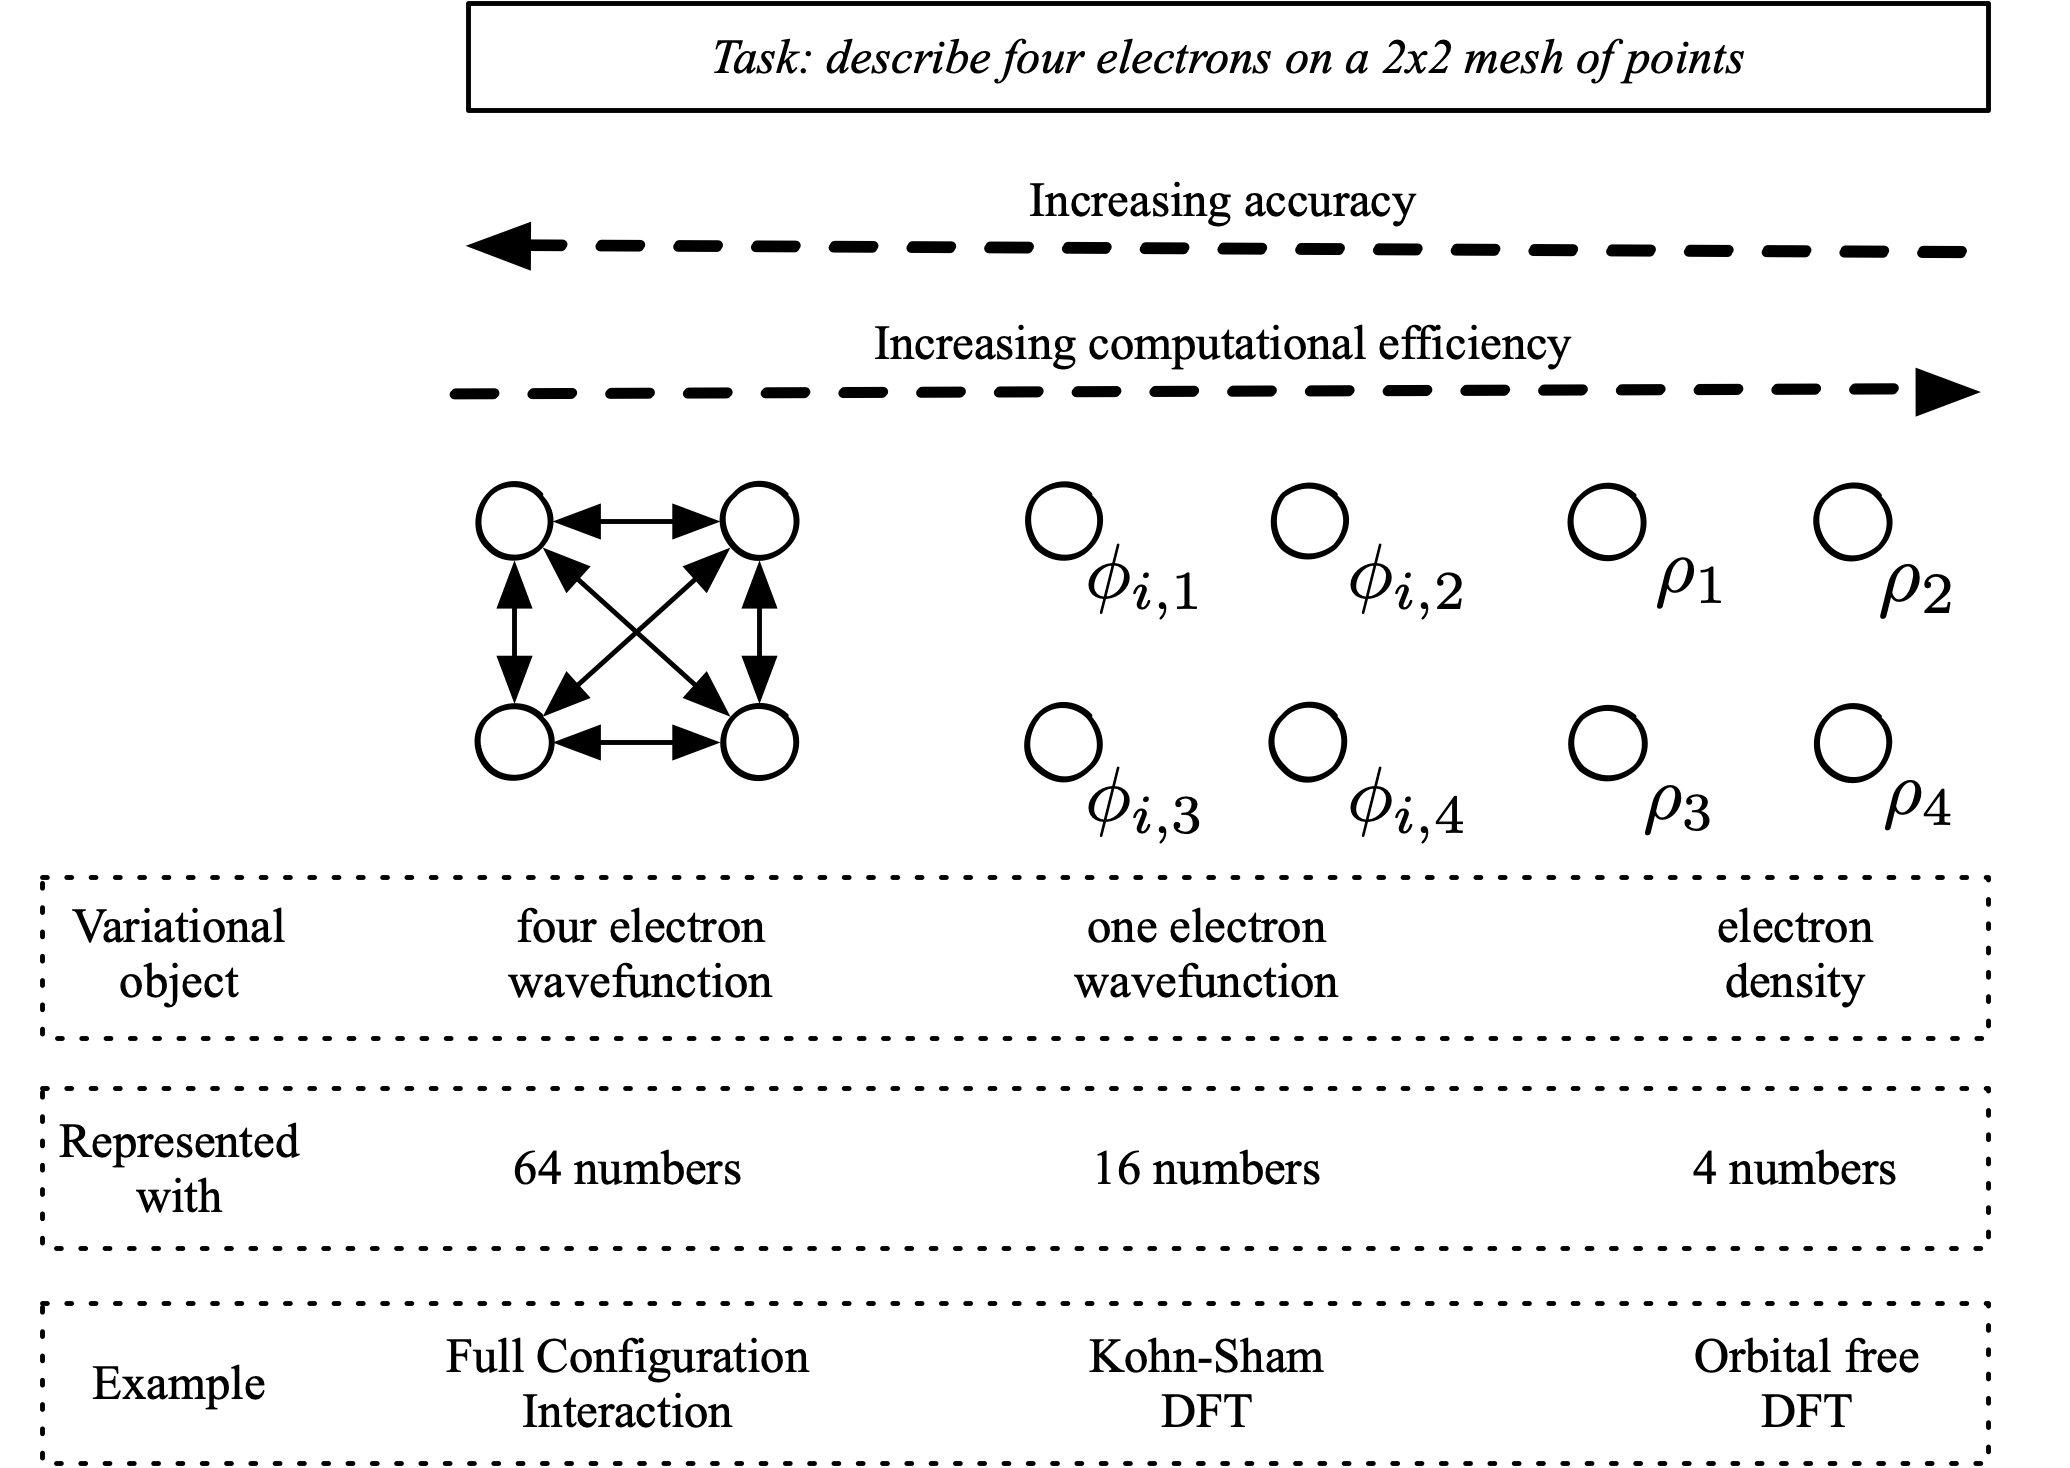
\includegraphics[width=0.8\columnwidth]{figures/ch3/dimensions.png}
  \caption[Dimensionality of variational objects]{To solve the Schr\"{o}dinger equation we can use a variational object with lower dimensionality and higher computational efficiency, although this will come at the cost of accuracy. This schematic is based on a discussion in Walter Kohn's Nobel Prize lecture.\autocite{Kohn1999}}
  \label{dimensions}
\end{figure}
% Is this right? I don't understand how the two electron wavefunction scales (4^2) - it's discussed in the 14 easy lessons.


\section{DFT in practice}

\subsection{Exchange-correlation functionals}
% explain here that Exc is defined by a difference in known energies, as is electron correlation
To use Kohn-Sham DFT we must approximate the exchange-correlation functional $E_{\textrm{xc}}\left[\rho\right]$, and there is a growing list of functionals at varying levels of complexity. John Perdew proposed `Jacob's Ladder' as a way to categorise these functionals (Figure \ref{jladder}). As a general rule, more accurate functionals are constructed by including more parameters and variables.

\begin{figure}[h]
\centering
  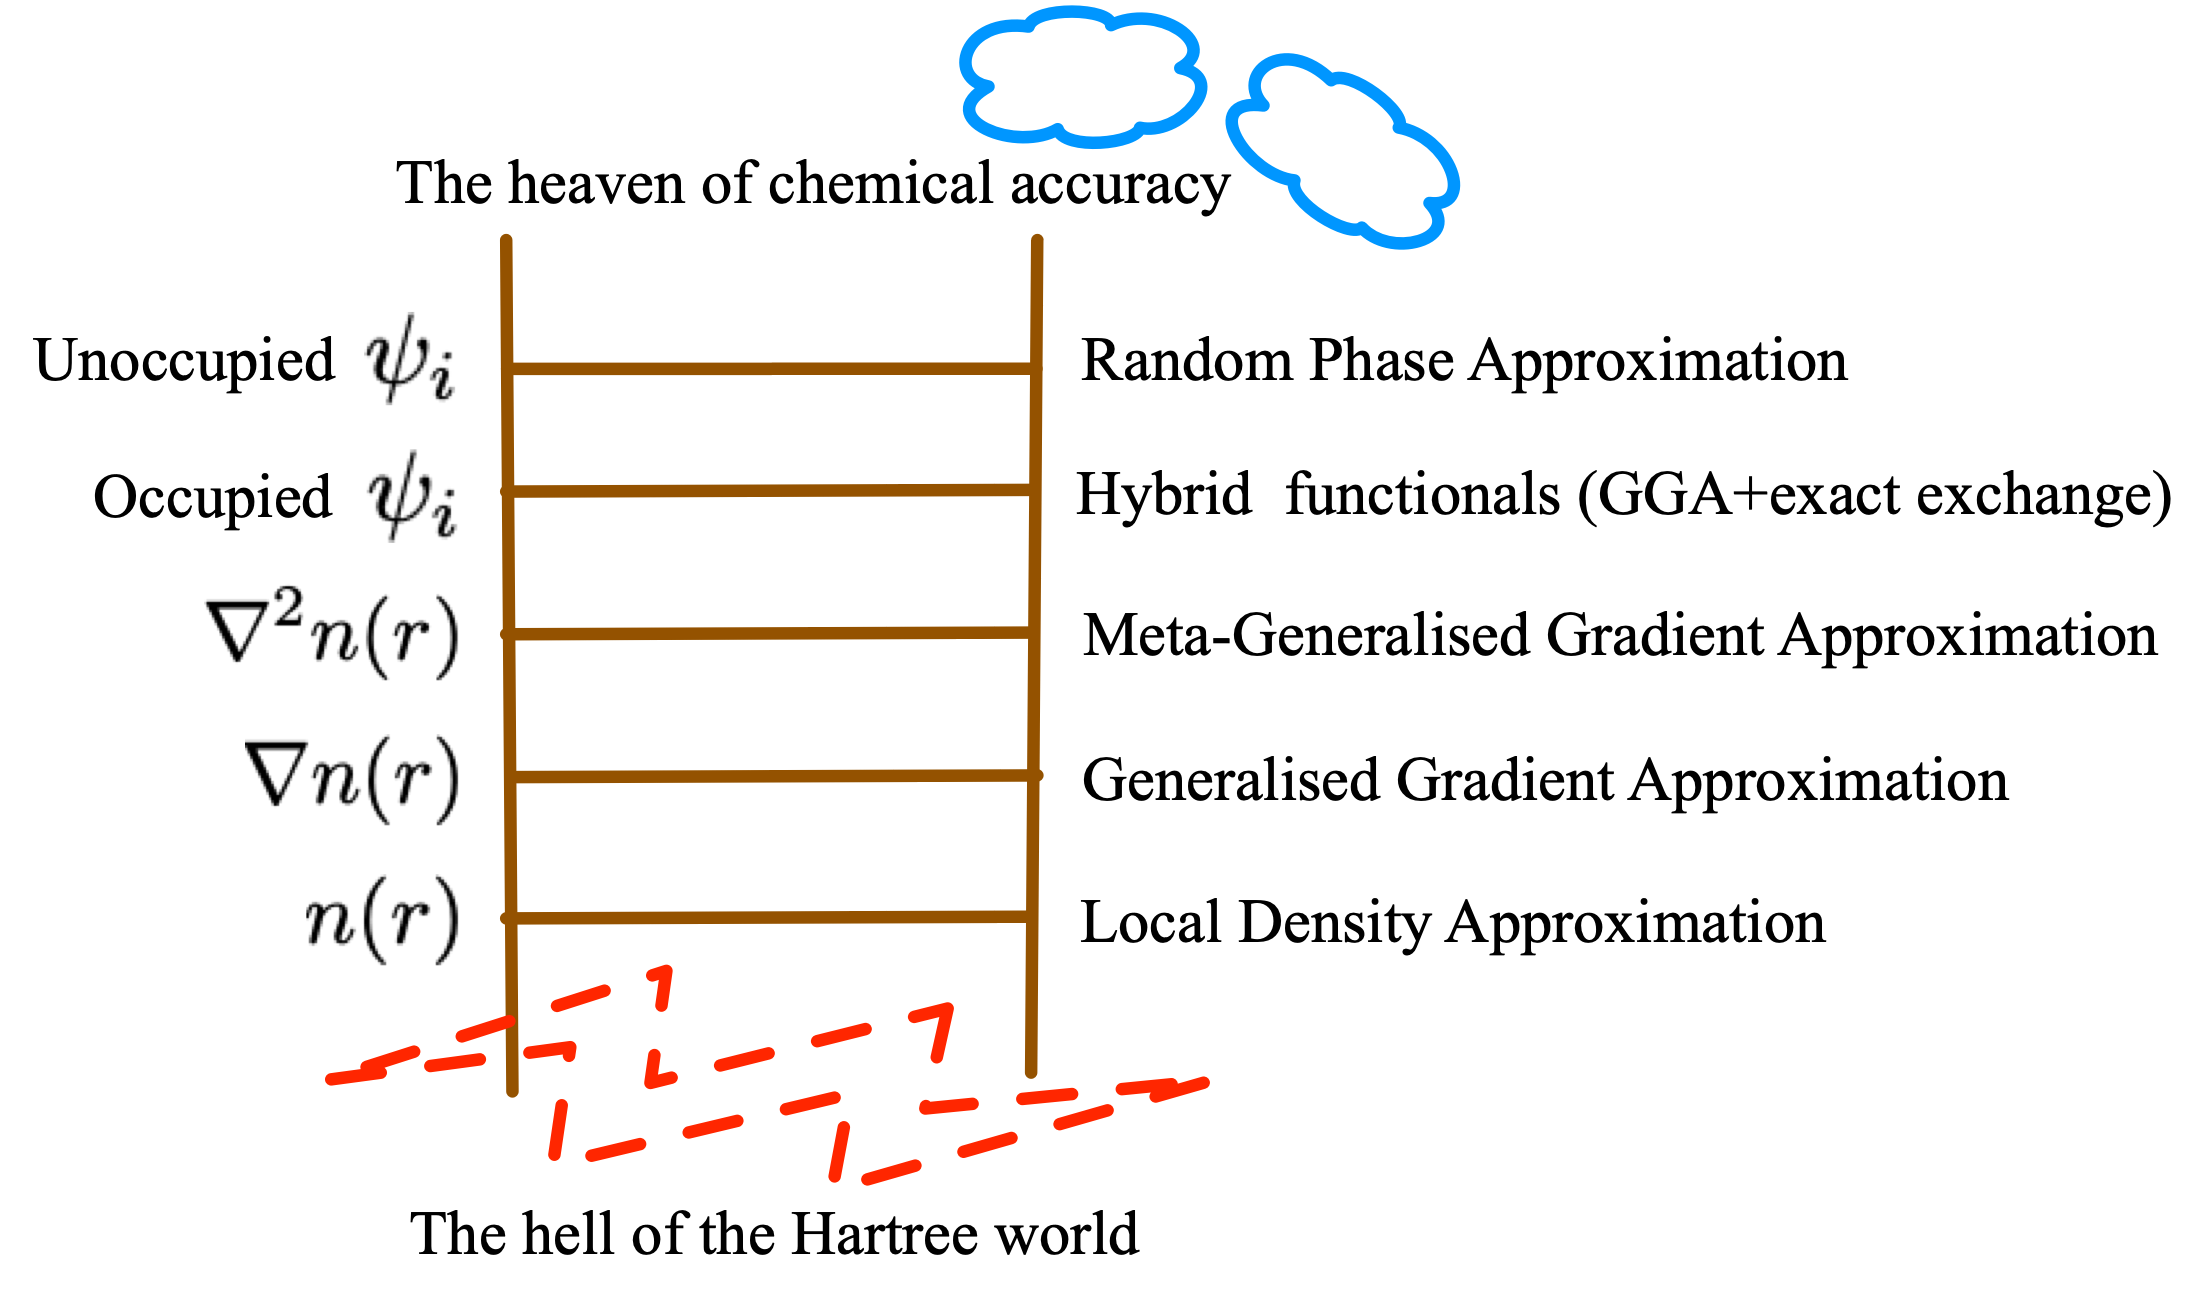
\includegraphics[width=0.8\columnwidth]{figures/ch3/jladder.png}
  \caption[Jacob's ladder of exchange-correlation functionals]{Jacob's ladder of exchange correlation functionals. On the right hand side are the various categories of exchange-correlation functionals and on the left hand side are the additional input variables included at each level of theory. As we move up the ladder the chemical accuracy increases, alongside computational expense.}
  \label{jladder}
\end{figure}


\textbf{Local Density Approximation} 

At the lowest rung of the ladder is the local density approximation (LDA) where only one variable, the electron density for an infinitesimal 3-dimensional volume element, is used to calculate the exchange correlation energy:\autocite{Henderson2008}
\begin{equation}
E_{\textrm{LDA,xc}} = \int E_{\textrm{HEG,xc}}\left[\rho\left(\textbf{r}\right)\right]\textrm{d}\mathbf{r} .
\end{equation}
It is assumed that the exchange-correlation energy density $E_{\textrm{HEG,xc}}$ is equal to that of a homogeneous electron gas (HEG) with identical electron density $\rho$. The exchange energy is calculated exactly:\autocite{Henderson2008}
\begin{equation}
E_{\textrm{HEG,x}}\left[\rho\left(\textbf{r}\right)\right] = -\frac{3}{4}\left(\frac{6}{\pi}\right)^{\frac{1}{3}} \rho^{\frac{4}{3}}\left(\textbf{r}\right),
\end{equation}
and the correlation energy is calculated numerically by fitting to many-body quantum Monte Carlo calculations for a homogeneous electron gas.\autocite{Ceperley1980} %Ceperley and Alder
Exchange and correlation effects are inherently non-local, and so we should not expect the LDA to give accurate results.  
However it has performed surprisingly well for predicting the properties of a variety of atoms, solids and molecules. This is due to a cancellation of errors: LDA underestimates the exchange energy and overestimates the correlation energy.\autocite{Burke2007} However there is a tendency for LDA to overestimate the binding energy and underestimate lattice parameters. This is a particularly pronounced problem in weakly bonded systems.

\textbf{Generalised Gradient Approximation}

At the next level of theory (generalised gradient approximation, GGA), two variables are used to determine the exchange-correlation energy: electron density and the density gradient. The LDA energy density is multiplied by a factor $F_\textrm{xc}$ which corrects for system inhomogeneities:\autocite{Henderson2008}
\begin{equation}
E_{\textrm{GGA,xc}} = \int  E_{\textrm{HEG,xc}}\left[\rho\left(\textbf{r}\right)\right]F_\textrm{xc}\left[\rho\left(\textbf{r}\right),\Delta\rho\left(\textbf{r}\right)\right]\textrm{d}\mathbf{r}.
\end{equation}
Due to their dependence on the electron density gradient, GGA functionals are classed as semi-local. The parameters of GGA functionals can be derived from physical constraints (a non-empirical approach, as in the widely used PBE functional), or obtained from fitting procedures (an empirical approach, as in the case of the B88 functional). GGAs improve the over-binding of LDA, but tend to underestimate the bandgap of the material.

\textbf{Hybrid functionals} 

In DFT each electron interacts with itself as the potential derives from the total charge density of the system. This error is particularly pronounced for localised states, for example after trapping an electron or hole at a defect site. Hybrid functionals combine the GGA functional exchange-correlation energy $E_{\textrm{GGA,xc}}$ with a proportion of the exact HF exchange energy $E_{\textrm{HF,x}}$ to partially correct the self-interaction error. The simplest hybrid functional takes the form:\autocite{Henderson2008}
\begin{equation} \label{simplehybrid}
E_{\textrm{hybrid,xc}} = \alpha E_{\textrm{HF,x}} + \left(1-\alpha\right)E_{\textrm{GGA,xc}}.
\end{equation}
In some studies the proportion of exact exchange is tuned to reproduce the property of interest correctly. For example, $\alpha=0.43$ is commonly used to correctly reproduce the bandgap of the hybrid halide perovskite MAPI.\autocite{Whalley2017} %

Range separated hybrid functionals are a generalisation of the above, without the requirement that $\alpha$ is constant.
To introduce range separated hybrids more formally we define the exchange-correlation hole $h_\mathrm{xc}$ as:
\begin{equation}
h_\mathrm{xc}(\mathbf{r}_1|\mathbf{r}_{12}) = \rho(\mathbf{r}_1|\mathbf{r}_{12})-\rho(\mathbf{r}_1),
\end{equation}
where $\rho(\mathbf{r}_1|\mathbf{r}_{12})$ is the probability density for simultaneously finding one electron at position $\mathbf{r}_1$ and another electron at a distance of $|\mathbf{r}_{12}|$.
The term \textit{hole} is used as $h_\mathrm{xc}$ describes the region in space around an electron in which the probability of finding another electron is close to zero.

The exchange-correlation hole for the simple hybrid functional (Equation \ref{simplehybrid}) is:\autocite{Henderson2008}
\begin{equation}
h_\mathrm{xc}(\mathbf{r}_1|\mathbf{r}_{12}) = \alpha h_{\textrm{HF,x}}(\mathbf{r}_1|\mathbf{r}_{12})+ \left(1-\alpha\right)h_{\textrm{GGA,x}}(\mathbf{r}_1|\mathbf{r}_{12}),
\end{equation}
whereas for range separated hybrid functionals the proportion of exact exchange used to determine the exchange-correlation hole depends upon the distance between the two electrons:\autocite{Henderson2008}
\begin{equation}
h_\mathrm{xc}(\mathbf{r}_1|\mathbf{r}_{12}) = \alpha(\mathbf{r}_{12}) h_{\textrm{HF,x}}(\mathbf{r}_1|\mathbf{r}_{12})+ \left(1-\alpha(\mathbf{r}_{12})\right)h_{\textrm{GGA,x}}(\mathbf{r}_1|\mathbf{r}_{12}).
\end{equation}
The hybrid functional HSE06\autocite{Heyd2003} is used to generate many of the results in this thesis. This is a screened range-separated functional where the exact exchange is used for small $\lvert\mathbf{r}_{12}\rvert$ only. 

%\textbf{Random Phase Approximation} 
%
%Closest to heaven is the Random Phase Approximation (RPA), which uses all of the Kohn-Sham orbitals (occupied and unoccupied) as input variables. The functionals listed so far are inaccurate when there are significant long range effects, as they have no information about the electron density far from an electron. The RPA is able to correctly predict long-range interactions, such as the van der Waals interaction, between non-overlapping electron orbitals.
% can I find plot of total energy as function of seperation using different approaches??
%As DFT is exact except for the approximation to the exchange-correlation functional, any shortcoming to a DFT prediction can be attributed to the XC-functional. It should be noted though that DFT 
% DFT was not designed to calculate bandgaps.
% - However, since 2000 functionals have been better at giving total energy but they don’t give accurate density: straying away from ab-initio into a fitting exercise: DFT is straying from the path towards an exact functional

\subsection{Periodicity and Bl\"{o}ch states} \label{periodicitysubsection}

The material studied in this thesis, MAPI, is a crystalline solid. Although we want to understand the properties of a finite piece of material, we use the standard approach and model the finite crystal as an infinite crystal. This is acceptable if the crystal piece is large enough so that its properties do not depend on size. Born-von Karman (periodic) boundary conditions are used so that the infinite crystal is built from a repeating array of unit cells. There are an infinite number of unit cells of different shapes and sizes that can be used to build an infinite crystal. Any physically significant function of the crystal must have the same periodicity.

When the Schr\"{o}dinger equation is solved for a single atom the solution gives wavefunctions corresponding to the 1$s$, 2$s$, 2$p$, etc orbitals found in chemistry. When the Schr\"{o}dinger equation is solved for a periodic system, wavefunctions are formed by Bl\"{o}ch functions $\psi_{\textbf{k}}$:\autocite{Hoffmann1987}
\begin{equation} \label{bloch}
\psi_{\textbf{k}} = u_\textbf{k}e^{i\textbf{k}\cdot\textbf{r}}.
\end{equation}   %could do a sketch of the two parts and the resulting part, and the periodic potential
The Bl\"{o}ch function is formed from the product of a basis function $u_\textbf{k}$ with the same periodicity as the crystal lattice, and a plane wave $e^{i\textbf{k}\cdot\textbf{r}}$. $\textbf{k}$ is the crystal wave vector which forms a space known as reciprocal space. To understand the physical significance of $\textbf{k}$ we consider an infinite 1D chain of hydrogen atoms separated at distance $L$. The electron states can be described as a linear combination of hydrogen 1$s$ orbitals $u_n$ centred at each lattice point:

\begin{equation} \label{1dbloch}
\psi_k = \sum_nu_ne^{iknL},
\end{equation}

where $k=0$ corresponds to the lowest energy in-phase state, and $k=\frac{\pi}{L}$ corresponds to the highest energy out-of-phase state.
Between these two extremes there is a continuum of states forming an electronic band (Figure \ref{bands}). 

For any periodic system we can apply the Schr\"{o}dinger equation for a specific $\textbf{k}$ and calculate the electronic bandstructure $E(\textbf{k})$. There are an infinite number of eigenvalues $E_n(\textbf{\textbf{k}})$, where $n$ is used to label a particular eigenvalue (band). As a result of crystal symmetry, $E_n(\textbf{k})$ is periodic and only $k$-vectors within a region of space known as the Brillouin zone ($|\textbf{k}|<\frac{\pi}{a}$) need to be considered.\autocite{Lundstrom2000} 
%talk about high symmetry points and the naming conventions (greek in zone and latin a boundaries) - choose route through use aflowlib

\begin{figure}[h]
\centering
  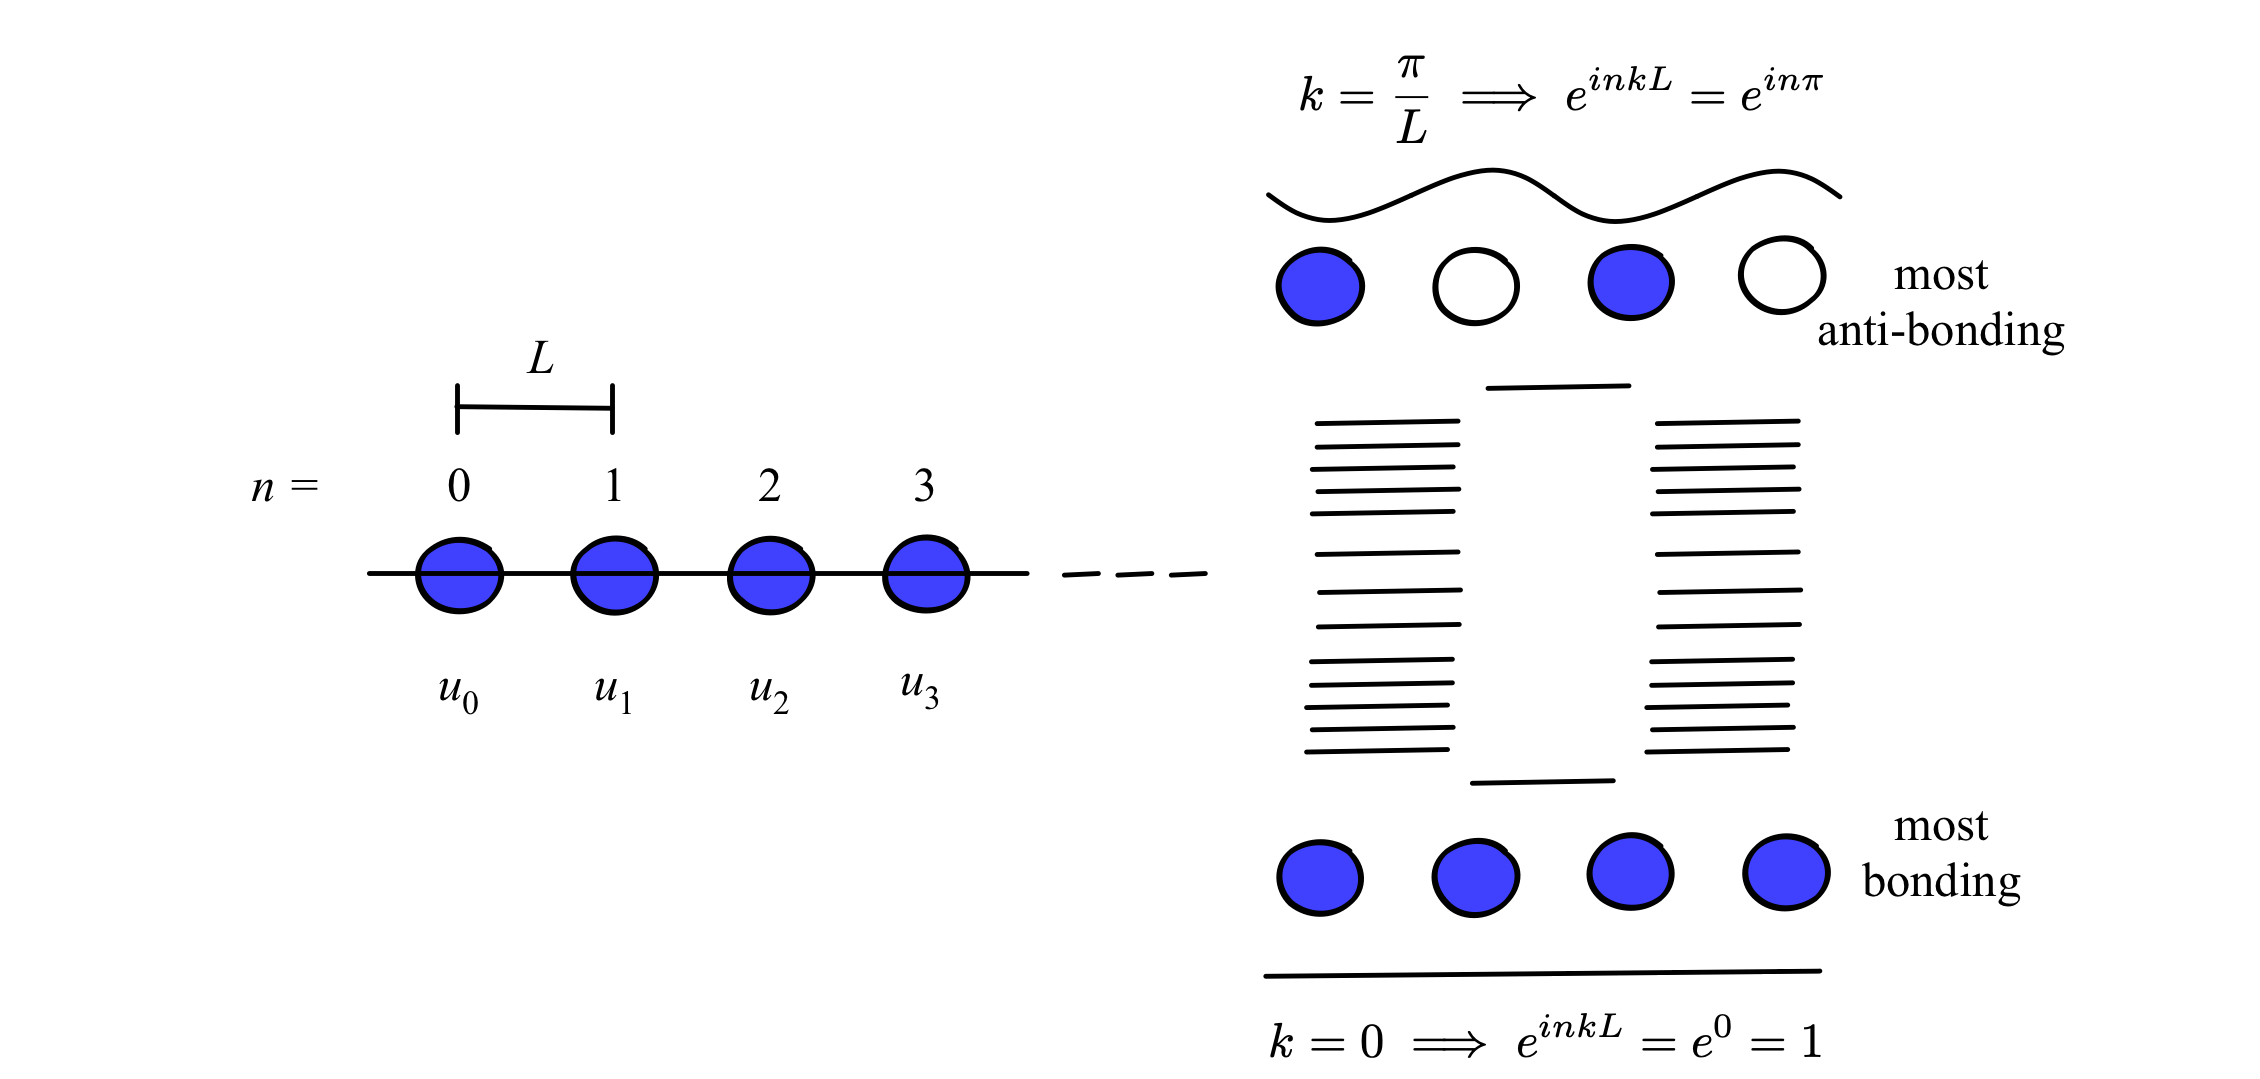
\includegraphics[width=1.0\columnwidth]{figures/ch3/bands.png}
  \caption[In-phase and out-of-phase states in an infinite 1D crystal]{(LHS) A one dimensional infinite chain of hydrogen atoms with index $n=0,1,2\ldots$. The atom spacing (unit cell length) is $L$, and there is a hydrogen 1$s$ orbital $u_n$ centred at each lattice point. The electron states for this system are formed from Bl\"{o}ch functions as given in Equation \ref{1dbloch}. (RHS) $k=0$ corresponds to a low energy in-phase state and $k=\frac{\pi}{L}$ corresponds to a high energy out-of-phase state. Between these two extremes there exists a continuum of states.} 
  \label{bands}
\end{figure}

In real materials translational symmetry can be broken, for example when there are point defects (as in Chapter \ref{ch:6-defects}). Furthermore, lattice vibrations have a periodicity larger than the unit cell. To model defects or lattice vibrations a supercell is built from multiple unit cells and this is used as the basic repeating unit cell (Figure \ref{translational}).

\begin{figure}[h]
\centering
  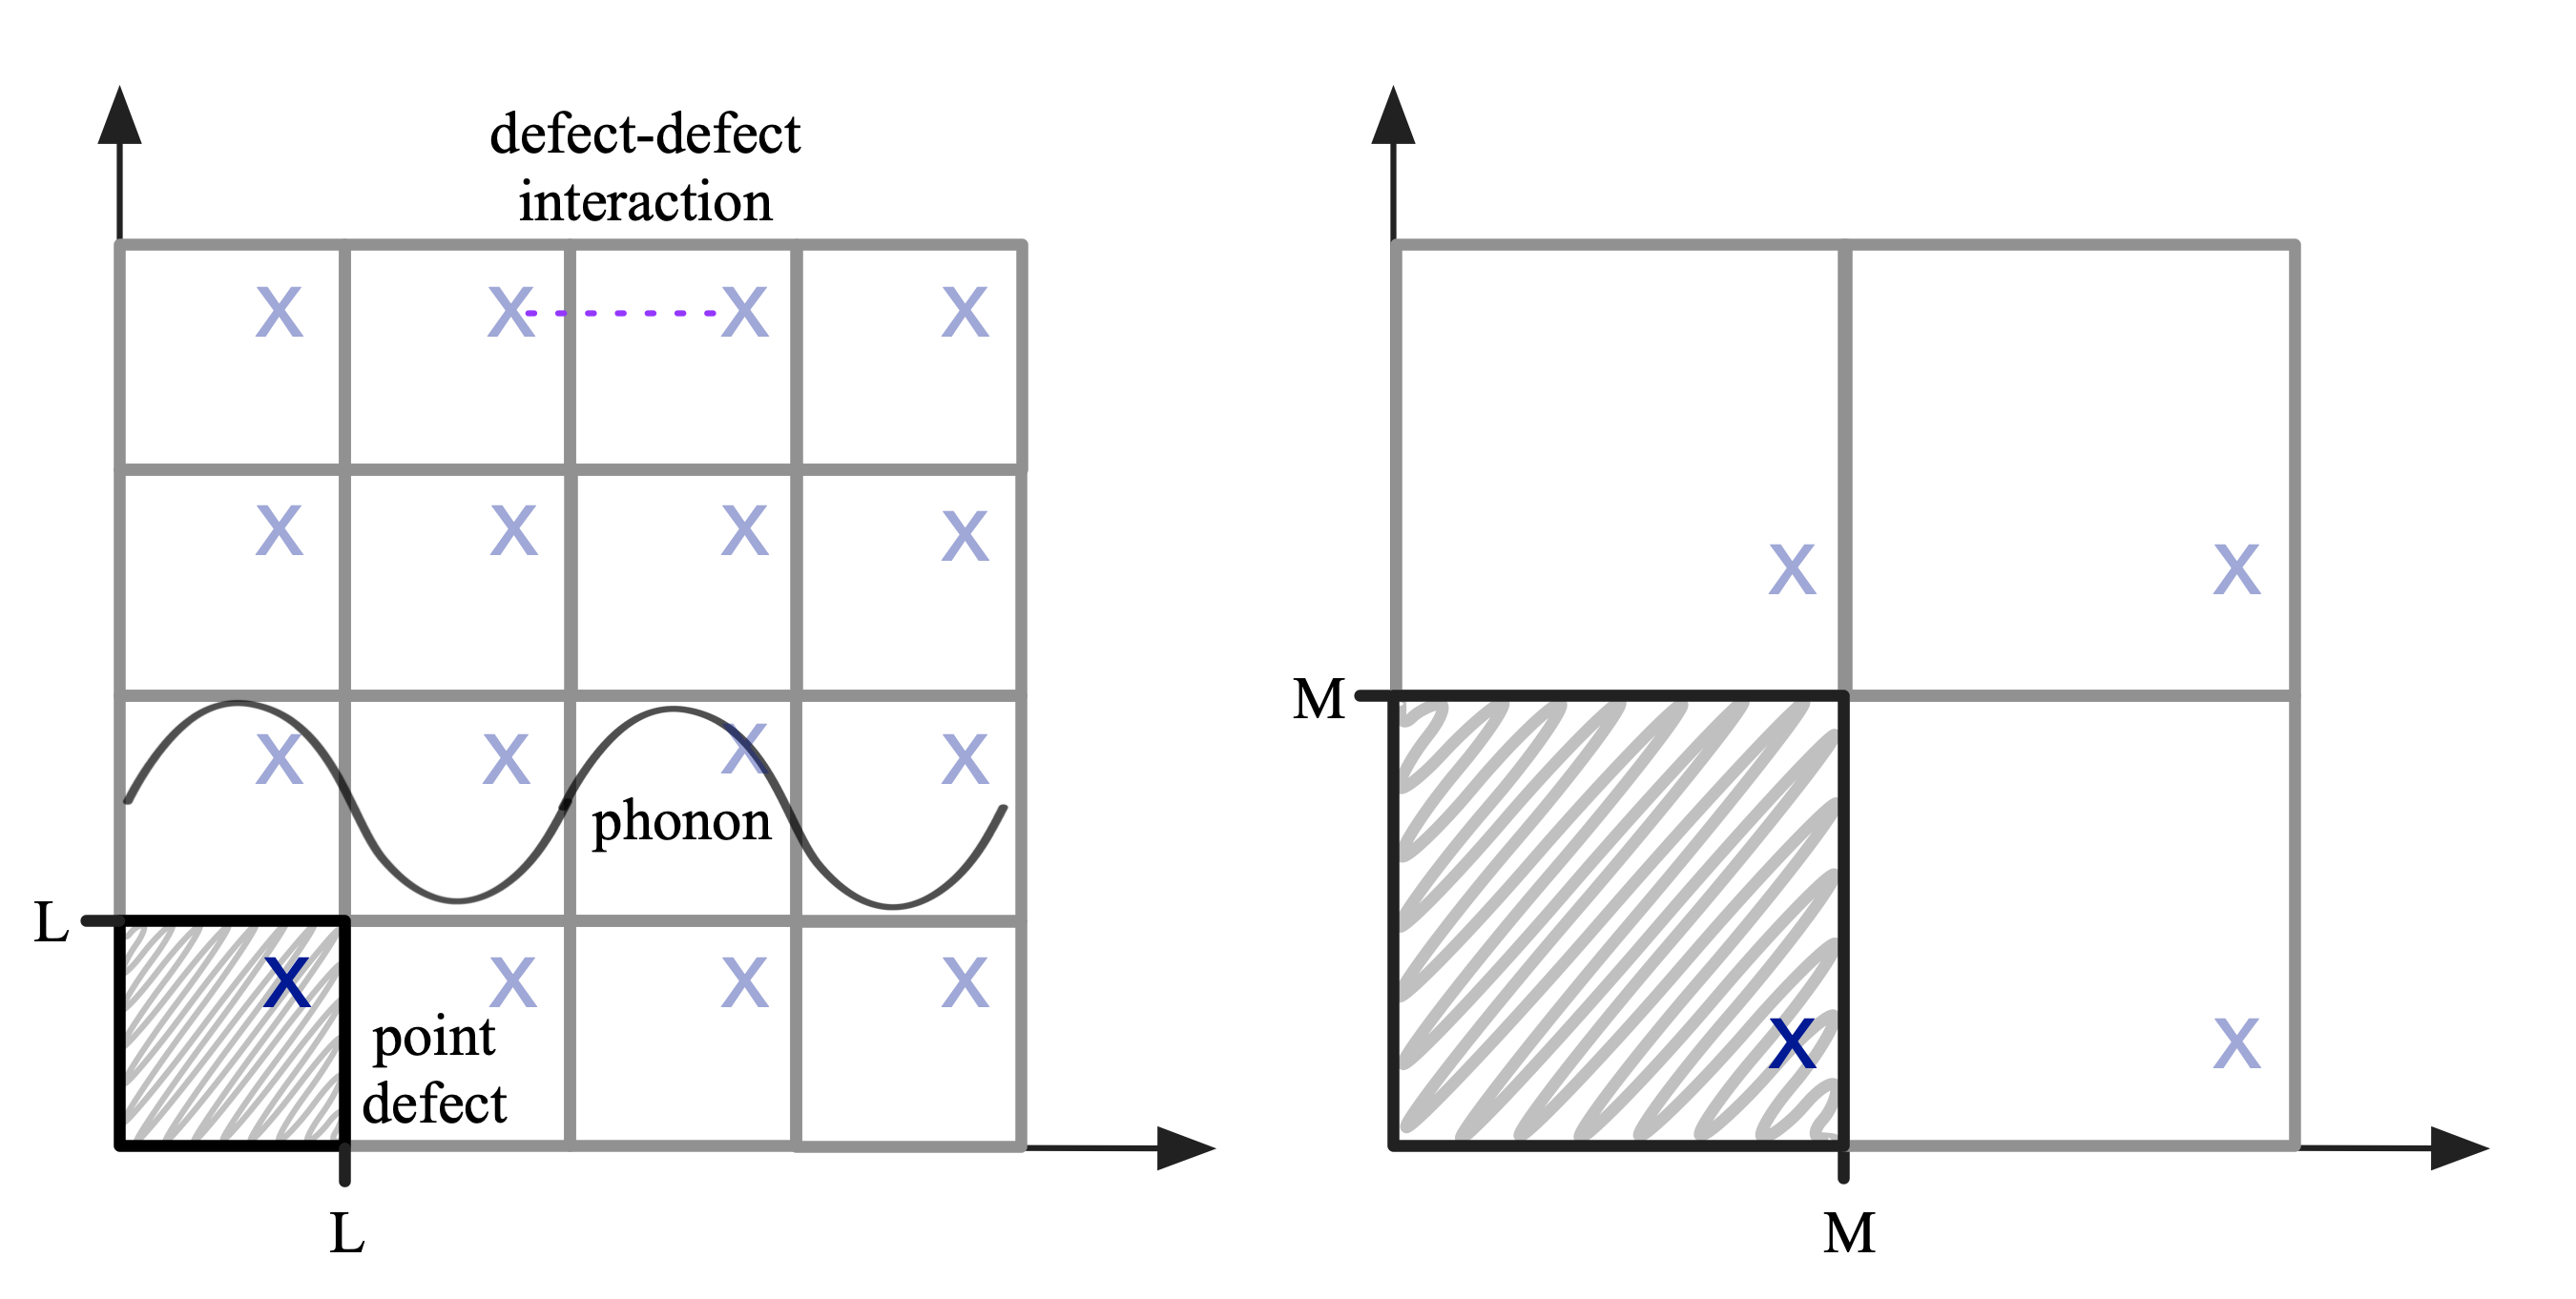
\includegraphics[width=0.8\columnwidth]{figures/ch3/supercell.png}
  \caption[Translational symmetry and supercell construction]{(LHS) An infinite crystal is built from a repeating unit cell of length $L$. Point defects (marked with an `x') break translational symmetey in real crystals and care must be taken when modelling these as neighbouring defects can interact with each other in an unphysical way. In addition, vibrational modes can have $\lambda>L$ (sine wave). (RHS) A supercell of length $M=2L$ can be built to reduce defect-defect interactions and model longer wavelength phonons. } 
  \label{translational}
\end{figure}

\subsection{Basis sets} \label{basissetsection}

In the previous section the Bl\"{o}ch wavefunction $\psi_\mathbf{k}$ was given for a 1D linear chain of hydrogen atoms, and the lattice periodic part of the Bl\"{o}ch function, $u_\mathbf{k}$, took the form of a hydrogen 1$s$ orbital. For more complex systems $u_\mathbf{k}$ can itself be expanded into a plane wave basis set:
\begin{equation}
u_\textbf{k} = \sum_\textbf{G}c_{\textbf{k},\textbf{G}}e^{i\textbf{G}\cdot\textbf{r}},
\end{equation}
where the wave vectors $\textbf{G}$ correspond to reciprocal lattice vectors and $u_\textbf{k}$ is the Fourier transformation of the wavefunction $\psi_\mathbf{k}$ in reciprocal space. 
As more terms are added to the Fourier series the electron density is described with increased accuracy.
Numerical convergence is used to justify the term at which the expansion is truncated (this is discussed further in Section \ref{numericalsubsection}).
The complete expanded wavefunction is:
\begin{equation} \label{KSeigenstates}
\psi_\textbf{k} = \sum_\textbf{G}c_{\textbf{k},\textbf{G}}e^{i(\textbf{k+G})\cdot\textbf{r}},
\end{equation}
where we see that the real space wavefunction has been mapped onto a series of plane waves in reciprocal space.

As a plane wave is inherently periodic this basis set is often used for extended systems. The software used for the DFT calculations in this thesis, \textsc{VASP},\autocite{Kresse1996} uses a plane wave basis set. For DFT calculations applied to localised systems, such as molecules or nanoparticles, localised basis sets such as gaussian orbitals are more likely to be used.

\subsection{Pseudopotentials}

Sudden changes in electron density are hard to capture using a plane wave basis set; to take an extreme example, the fourier decomposition of a simple top hat in real space requires an infinite summation in reciprocal space. This can be problematic when describing the region around the nucleus where there are strong oscillations in the DFT wavefunctions. Instead, pseudopotentials - effective potentials which do not lead to oscillations in the wavefunction - can be used. It has been established that for certain systems pseudopotentials are as precise as all-electron calculations.\autocite{Lejaeghere2016}

To develop a pseudopotential for a particular element we consider it as an isolated atom and split the single-particle electron states into a set of valence states $\{\psi^\mathrm{v}\}$ and core states $\{\psi^\mathrm{c}\}$.\autocite{Kaxiras2007} The core states are those which contribute a negligible amount to the total electron density beyond a cutoff radius $r_c$. Both sets of states satisfy the single-particle Schr\"{o}dinger equation for the atom:
\begin{align} \label{speqn}
\hat{H}\psi^\mathrm{v} = \epsilon^\mathrm{v}\psi^\mathrm{v} \\
\hat{H}\psi^\mathrm{c} = \epsilon^\mathrm{c}\psi^\mathrm{c},
\end{align}
where $\hat{H}$ contains a potential $V$ which accounts the electron-ion and electron-electron interactions.

A new set of single particle valence states, $\{\tilde{\psi}^\mathrm{v}\}$ can be defined so that they obey the single-particle Schr\"{o}dinger equation above, but now with an additional potential term $\tilde{V}$. 
The pseudopotential $V_\mathrm{ps}$ is the modified potential which includes this term.
In addition, the valence states $\{\tilde{\psi}^\mathrm{v}\}$ are constructed so that: 1) they have zero overlap with the core states $\{\psi^\mathrm{c}\}$; 2) their eigenvalues (for the modified Hamiltonian) are equal to $\epsilon^\mathrm{v}$; and 3) the additional $\tilde{V}$ term is repulsive.

The repulsive $\tilde{V}$ term can can be interpreted as the core electrons shielding the valence electrons from the attractive Coulomb potential of the atom. For a mathematical description of the pseudpotential construction process the reader is referred to Chapter 2 of Reference \cite{Kaxiras2007}.

The pseudopotential $V_\mathrm{ps}$ is not unique, and is constructed so that $\{\tilde{\psi}^\mathrm{v}\}$ reproduce the behaviour of $\{\psi^\mathrm{v}\}$ beyond the cutoff radius $r_c$. Within this radius, where the behaviour of the wavefunction does not determine the properties of a solid, the $\{\tilde{\psi}^\mathrm{v}\}$ are designed to be smooth and nodeless (Figure \ref{ppfigure}).

\begin{figure}[h]
\centering
  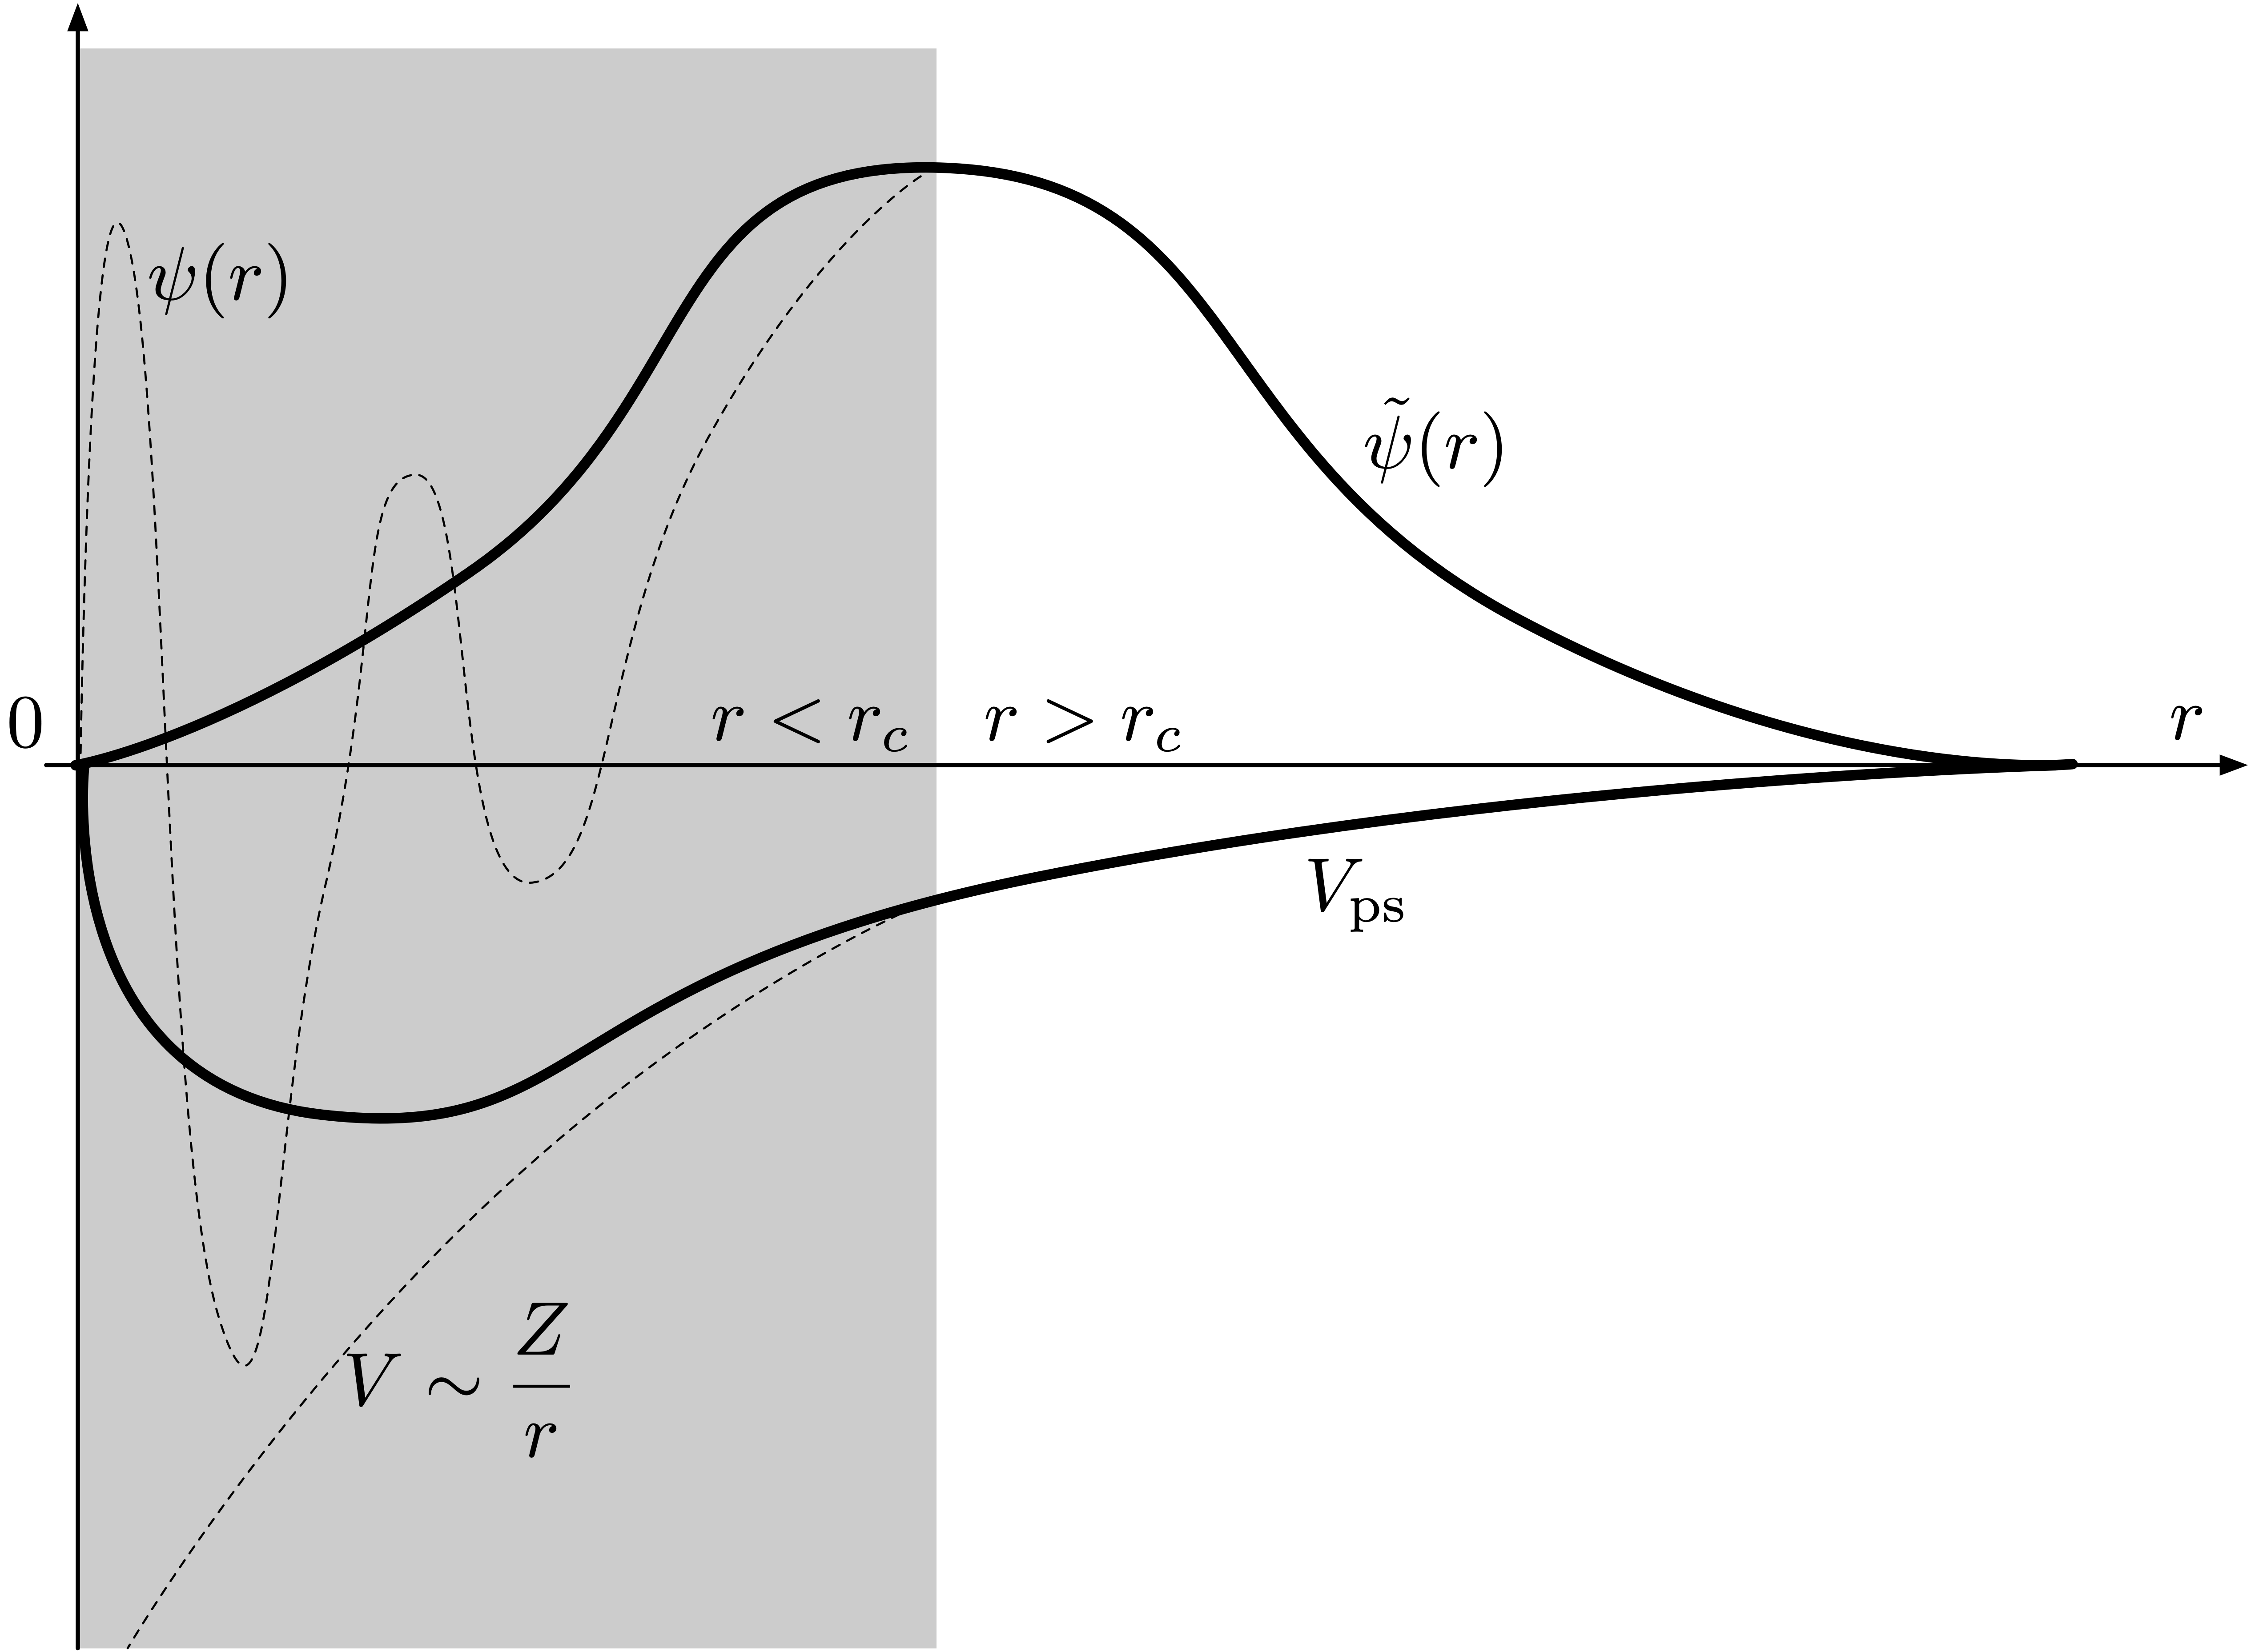
\includegraphics[width=0.6\columnwidth]{figures/ch3/ppfigure.png}
  \caption[Construction of the pseudo-wavefunction and pseudopotential]{Construction of the pseudo-wavefunction $\tilde{\psi}$ and pseudopotential $\tilde{V}$. Within the cutoff radius $r_c$ the pseudo-wavefunction is smooth and nodeless. As a result the pseudopotential is finite and smooth near the origin, instead of having a singularity like the Coulomb potential. Beyond $r_c$ the pseudo-wavefunction and pseudopotential reproduce the atomic wavefunction $\psi$ and Coulomb potential of the ion, respectively.}
  \label{ppfigure}
\end{figure}

The key benefits of the pseudopotential method are that: 1) the size of the basis set needed to expand the wavefunctions is reduced (as the strong oscillations within the core region are removed); and 2) it can be combined with the `frozen core' approximation so that the Kohn-Sham equations are solved for the valence electrons only. Both of these features reduce the computational cost of an electronic structure calculation.

There are several flavours of pseudopotential. Norm-conserving pseudopotentials are constructed so that within $r_c$ the norm of $\tilde{\psi}^\mathrm{v}$ is identical to that of the corresponding state $\psi^\mathrm{v}$. This constraint increases the computational cost for first row elements and transition metals. Ultrasoft pseudopotentials (USPP) do not enforce conservation of the norm, which allows for a reduction in basis set size. The projector augmented wave approach combines the pseudopotential method with the linear augmented plane wave method.\autocite{Blochl1994} The resulting pseudopotentials provide access to the full wavefunction (rather than the wavefunction beyond $r_c$) at a cost comparable to the construction of USPP.


%http://helper.ipam.ucla.edu/publications/maws3/maws3_6085.pdf
%http://davidbowler.github.io/AtomisticSimulations//blog/dft-reliability#R3

\subsection{Optimising the atomic and electronic structure} \label{SCFsubsection}

In this section the process of optimising the atomic and electronic structure of a system towards the ground-state (minimum energy) configuration is outlined. 

As outlined in Section \ref{KSformalismsubsection}, the Coulomb and exchange-correlation potentials are dependent on the electron density $\rho(\mathbf{r})$, which is itself dependent on the potentials. Therefore an iterative approach called the self consistent field method is used to calculate the ground-state electronic structure (Figure \ref{SCF}, dashed section). An initial guess for the density $\rho(\textbf{r})$ is given by a superposition of the atomic charge densities. This is used to calculate the potential and solve the KS equations, which gives a new $\rho(\textbf{r})$. This process continues until there is convergence within a given energy tolerance. Various optimisation routines are provided in DFT codes for finding the ground state configuration, including the conjugate gradient scheme, Davidson Scheme and RMM-DIIS.

DFT is also used to find the ground state atomic structure. Structures inferred from X-ray diffraction data are used as a starting guess, so that finding the energetic minimum becomes a local optimisation problem. Atoms in the systems are displaced (either the internal coordinates of the unit cell or the unit cell parameters themselves are adjusted) and the electronic structure for that geometry is solved self-consistently. This process repeats until the forces on each atom are zero to within a given tolerance (Figure \ref{SCF}). 

\begin{figure}[h]
\centering
  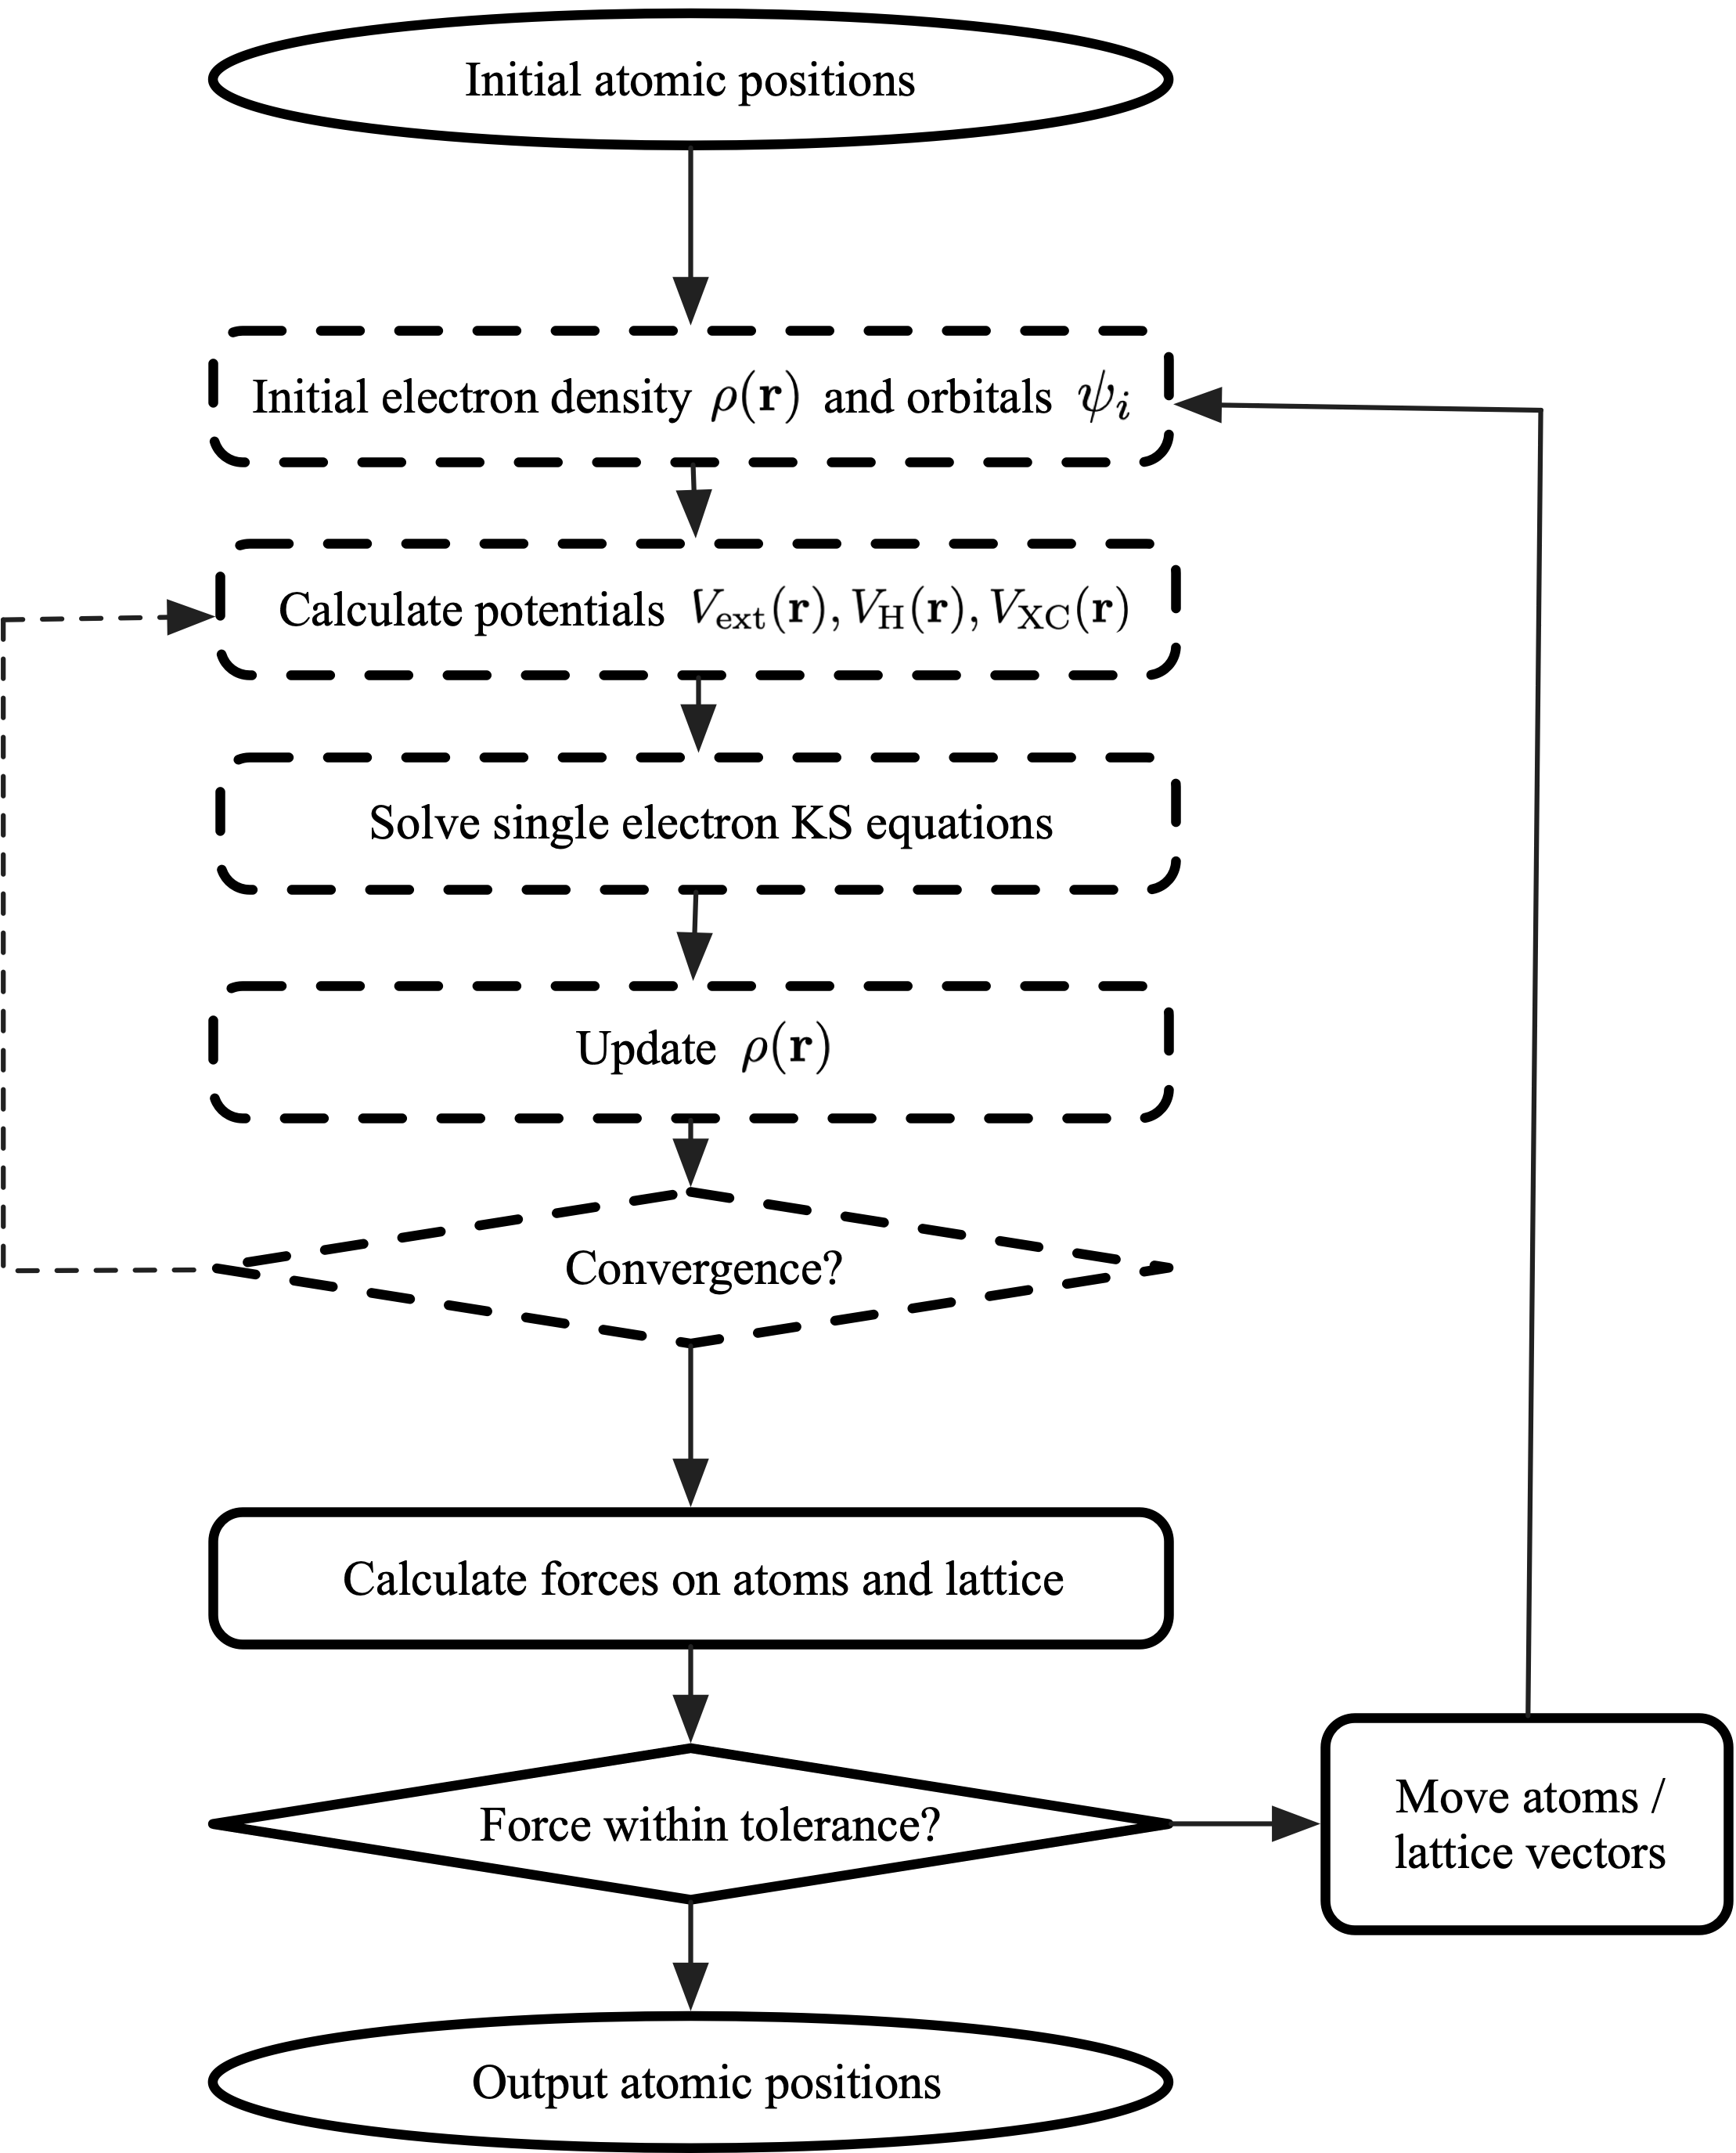
\includegraphics[width=0.7\columnwidth]{figures/ch3/scf.png}
  \caption[Nested iterative method for geometry optimisation]{Nested iterative method for geometry optimisation. The electronic structure relaxation (dashed lines) is nested within the atomic structure relaxation (solid lines). $v_\textrm{ext}(\textbf{r})$, $v_\textrm{c}(\textbf{r})$ and $v_\textrm{xc}(\textbf{r})$ correspond to the external, classical (electrostatic) and exchange-correlation potentials respectively.} 
  \label{SCF}
\end{figure}

\subsection{The limits of DFT} \label{numericalsubsection}


\textbf{Theoretical limitations} 

In Section \ref{DFTtheory} the approximations inherent to DFT calculations were outlined: the Born-Oppenheimer approximation and the unknown exchange-correlation functional. Higher levels of theory, which incorporate the effects of spin and relativity (e.g. spin-orbit coupling) are included in many DFT implementations. However DFT is still restricted to ground-state properties and higher levels of theory (GW or time-dependent DFT) are required to describe excited states. Another inherent limitation is that the KS eigenvalues are artificial; only the ground state electron density and derived properties are correct. In practice the KS eigenvalues are used to calculate the bandgap, but quantitatively correct bandgaps often require the use of hybrid functionals with empirically-set parameters.

\textbf{Numerical limitations} 

There are also approximations that relate to numerical convergence rather than the underlying theory.
In Section \ref{basissetsection} we expanded the lattice periodic part of a wavefunction into a plane wave basis set. In principle an infinite set may be needed to describe the orbitals, but in practice the basis set must be truncated. The kinetic energy operator is given by $-\frac{\hbar^2 }{2m}\nabla^2$ and when this is applied to the wavefunction $\psi_\mathbf{k}$ as given in Equation \ref{KSeigenstates}, we find that the kinetic energy is proportional to $|\mathbf{k}+\mathbf{G}|^2$; faster plane-wave oscillations correspond to higher energies. A cutoff energy $\textrm{E}_\textrm{cut}$ is defined so that
\begin{equation}
\frac{1}{2}|\mathbf{k}+\mathbf{G}|^2 < \textrm{E}_\textrm{cut}.
\end{equation}
This cutoff energy must be tested to ensure that the property of interest (which is often energy) is converged to within a certain tolerance.

To calculate many material properties we need to integrate over the Brillouin zone in reciprocal space. To calculate the total energy of an insulator for example, we use
\begin{equation} \label{energyintegral}
    E = \frac{\Omega}{(2\pi)^3}\sum_\textrm{occ.}\int_\textrm{BZ}E(\textbf{k})d^3k
\end{equation}
where $\Omega$ is the volume of the Brillouin zone and the sum is over all occupied bands. 
In practice we do not know the continuous form for $E(\textbf{k})$ and so we numerically evaluate Equation \ref{energyintegral} as a weighted sum over special points in reciprocal space. These points often form an equally spaced mesh centred on the $\Gamma$-point ($\textbf{k}=(0,0,0)$) in reciprocal space. For any given system, the $k$-point density scales inversely with cell size; for example, if the unit cell in Figure \ref{translational} requires a $6\times6$ $k$-point grid, then the larger $2\times2$ supercell requires a $3\times3$ $k$-point grid. As with plane waves, there is a balance between accuracy (the higher the number of $k$-points, the higher the accuracy) and computational expense. An example convergence study is given in Figure \ref{kpointconvergence} where a $5\times5\times5$ $k$-point grid is required to converge pressure to within \SI{1}{\kilo\bar} and energy to within \SI{0.1}{\electronvolt}.

\begin{figure}[h]
\centering
  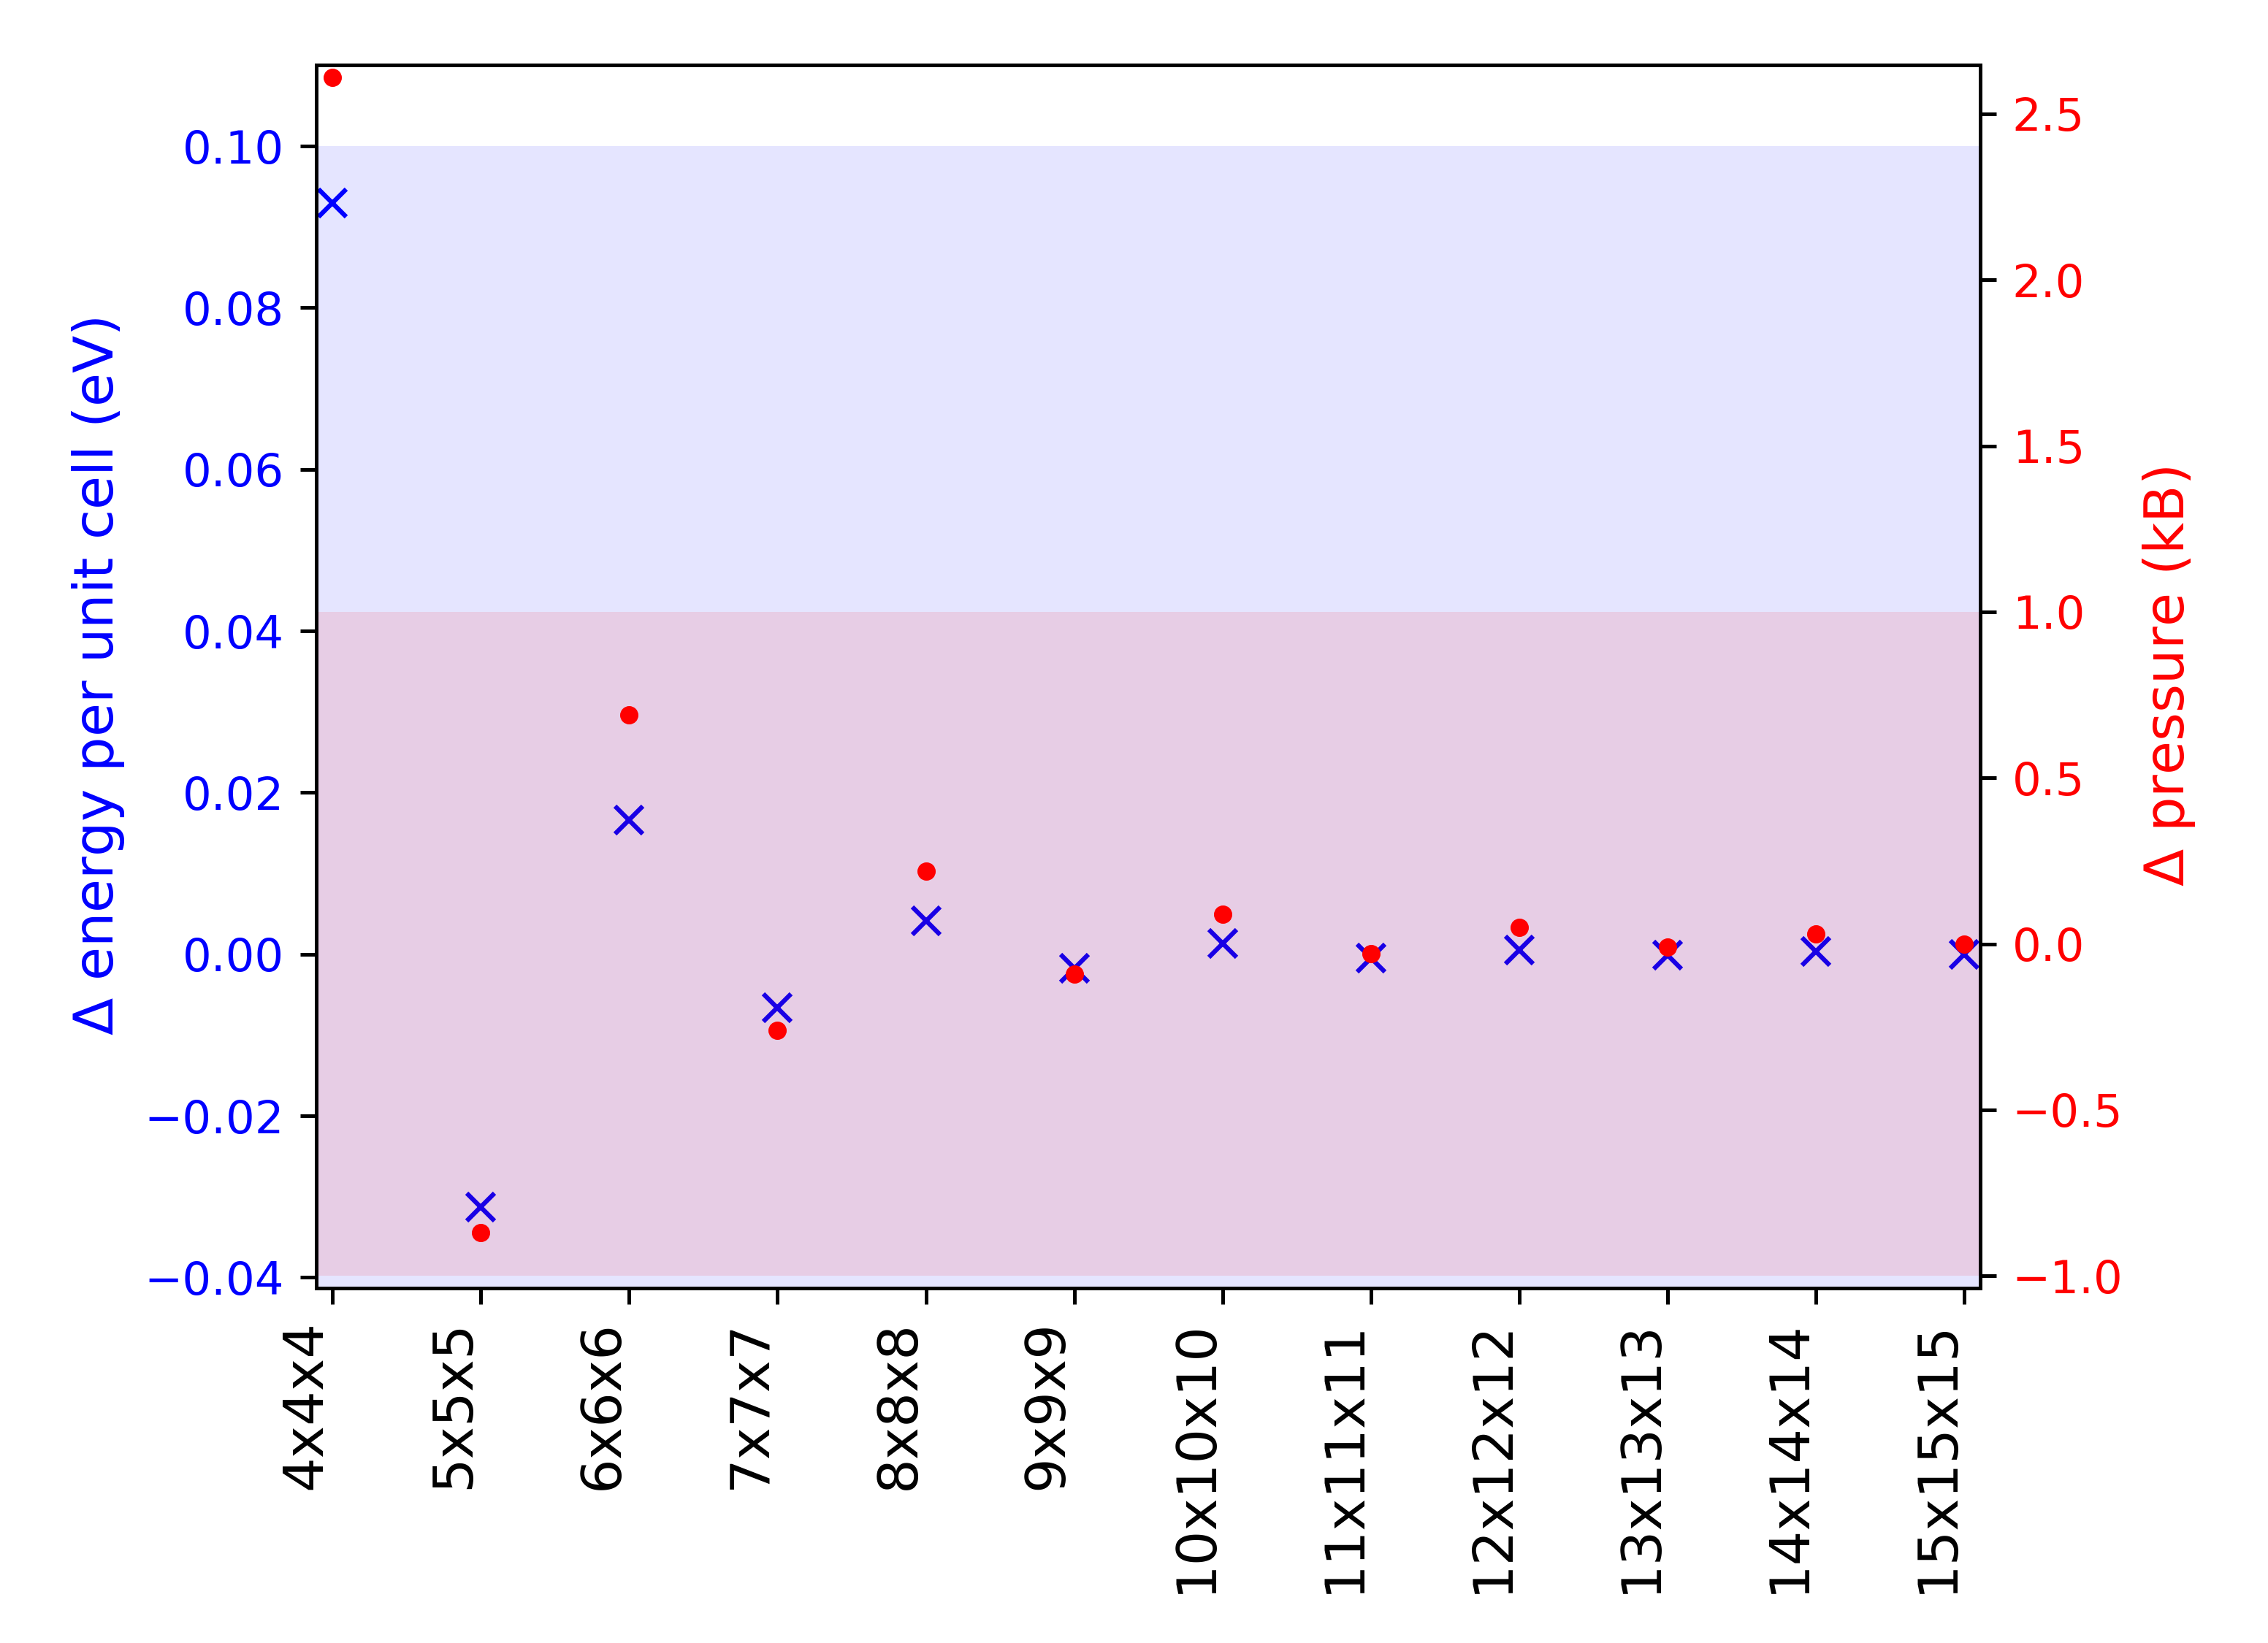
\includegraphics[width=0.7\columnwidth]{figures/ch3/kpointconvergence.png}
  \caption[\ce{CsSnI3} $k$-point convergence]{$k$-point convergence of \ce{CsSnI3}. The $k$-point grid size is on the $x$-axis. Red dots denote pressure; the region which is within the convergence criteria of \SI{1}{\kilo\bar} is shaded red. Blue crosses denote total energy; the region which is within the \SI{0.1}{\electronvolt} convergence criteria is shaded in blue. Only odd grids sample the $\Gamma$-point and so there is an oscillation in energy and pressure as points move between odd and even grids.}
  \label{kpointconvergence}
\end{figure}


% - K-point grids and the commensurate grids for supercells.
% - Doubles k-points reuired as k and –k now no longer equivalent (SoC?)
%All convergence tests must be done for the property of interest. Cancellation of errors can mean that energy differences converge faster than ground state energies, as is reported in Chapter \ref{}.   % EP coupling calcas 
% - See: Designing meaningful density functional theory calculation in materials science - a primer Anne E Mattson et al. Model. Sim. Mater. Sci Eng. 13 R1-R31 (2005). : for information about convergence and getting meaningful results.

%\textit{Computational limitations}
% - history of computers section at science museum for HPC section
% - put the amount of computer time and carbon burnt here?
% - computational expense: limitations on size: See review of materials models which Alison Walker mentions. Mesoscopic bridges the atomistic with the drift diffusion models. Meso is often monte carlo, tranjectory tpe calculations. Cells are too big for atomistic (1 cm squared). Efficiecny depends upon J-V curves which can only be modelled at scale of fill device. The electrostatics is incredible important which linked ot build up of charges at SC nd OC. Grain boundaries and recombination at intercaes.

\section{Defects in semiconductors}

The second law of thermodynamics states that an isolated system tends towards an equilibrium state with maximum entropy. A consequence of this is that all solids in equilibrium and at finite temperature contain point defects, as the cost in lattice energy is balanced by the increase in configurational entropy. 
Point defects are associated with a number of microscopic processes that can be either beneficial or detrimental to material performance, including:
\setlist{nolistsep}
\begin{itemize}[noitemsep]
    \item optical: colour centres, up/down conversion
    \item electrical: conductivity, carrier trapping, ionic hopping
    \item mechanical: material hardening
    \item thermal: conductivity, decomposition
\end{itemize}
%Yakov Frenkel introduced the concept of defects in a crystalline structure in 1926. Research interest in this field continued throughout the 20th and 21st centuries as the physical processes listed above determine the success or failure of technologically important materials. 
Theoretical methods are particularly useful in this area as although it is often possible to estimate the quantity of defects in a material using experimental methods, it is much more challenging to identify the defect species.\autocite{Alkauskas2016}  
 
In this section I outline the different types of crystal defects and discuss the thermodynamics of (charged) defect formation. The supercell method for calculating defect properties is also outlined. This method is used in Chapter \ref{ch:6-defects}.
% We are interested in calculating the electronic structure properties which lead to a description of the defects (trap density, binding energy, trap level, capture cross section).

% cite defects and defect processes in nonmetallic solids

% - History:
% - 1912 Born and Karman . PBC (first lattice dynamics paper)
% - 1925 Frenkel – formation of frenkel pair (first defects paper)
% - 1922 Jost – probability of forming defects. Tied into experimental work popular at the time, looking at how a material can be an ionic conductor when it is electrically insulating
% - 1938 Mott – the Mott-Littleton approach for calculating defects

\subsection{Classification of crystal defects}

The first way to classify defects is via their dimensionality. 0-dimensional point defects are localised around isolated sites in the crystal. 1-dimensional dislocations are lines along which the crystal pattern is broken. 2-dimensional grain boundaries or interfaces are surfaces along which distinct crystallites are joined. 3-dimensional defects are changes to the crystal pattern in a finite volume. 

0-dimensional point defects are the subject of Chapter \ref{ch:6-defects}. Point defects can be further split into extrinsic or intrinsic defects. Extrinsic point defects (also known as impurities) are a different species from that of the host. These defects may be added intentionally (for example, to increase electrical conductivity) or unintentionally (as a result of the fabrication method). Intrinsic point defects are associated with the host species.

Point defects can also be classified as non-stochiometric or stochiometric. Non-stochiometric defects include interstitials (where an additional atom occupies a site that is unoccupied in the perfect lattice), vacancies (missing atoms) and antisites (where an atom occupies a site that would have been occupied by another species in the perfect lattice). Interstitials can have a split structure, in which two atoms are split symmetrically around a single lattice site. Stochiometric defects include Frenkel pairs and Shottky pairs. Stochiometric and non-stochiometric point defects are illustrated in Figure \ref{classification}.

\begin{figure}[h]
\centering
  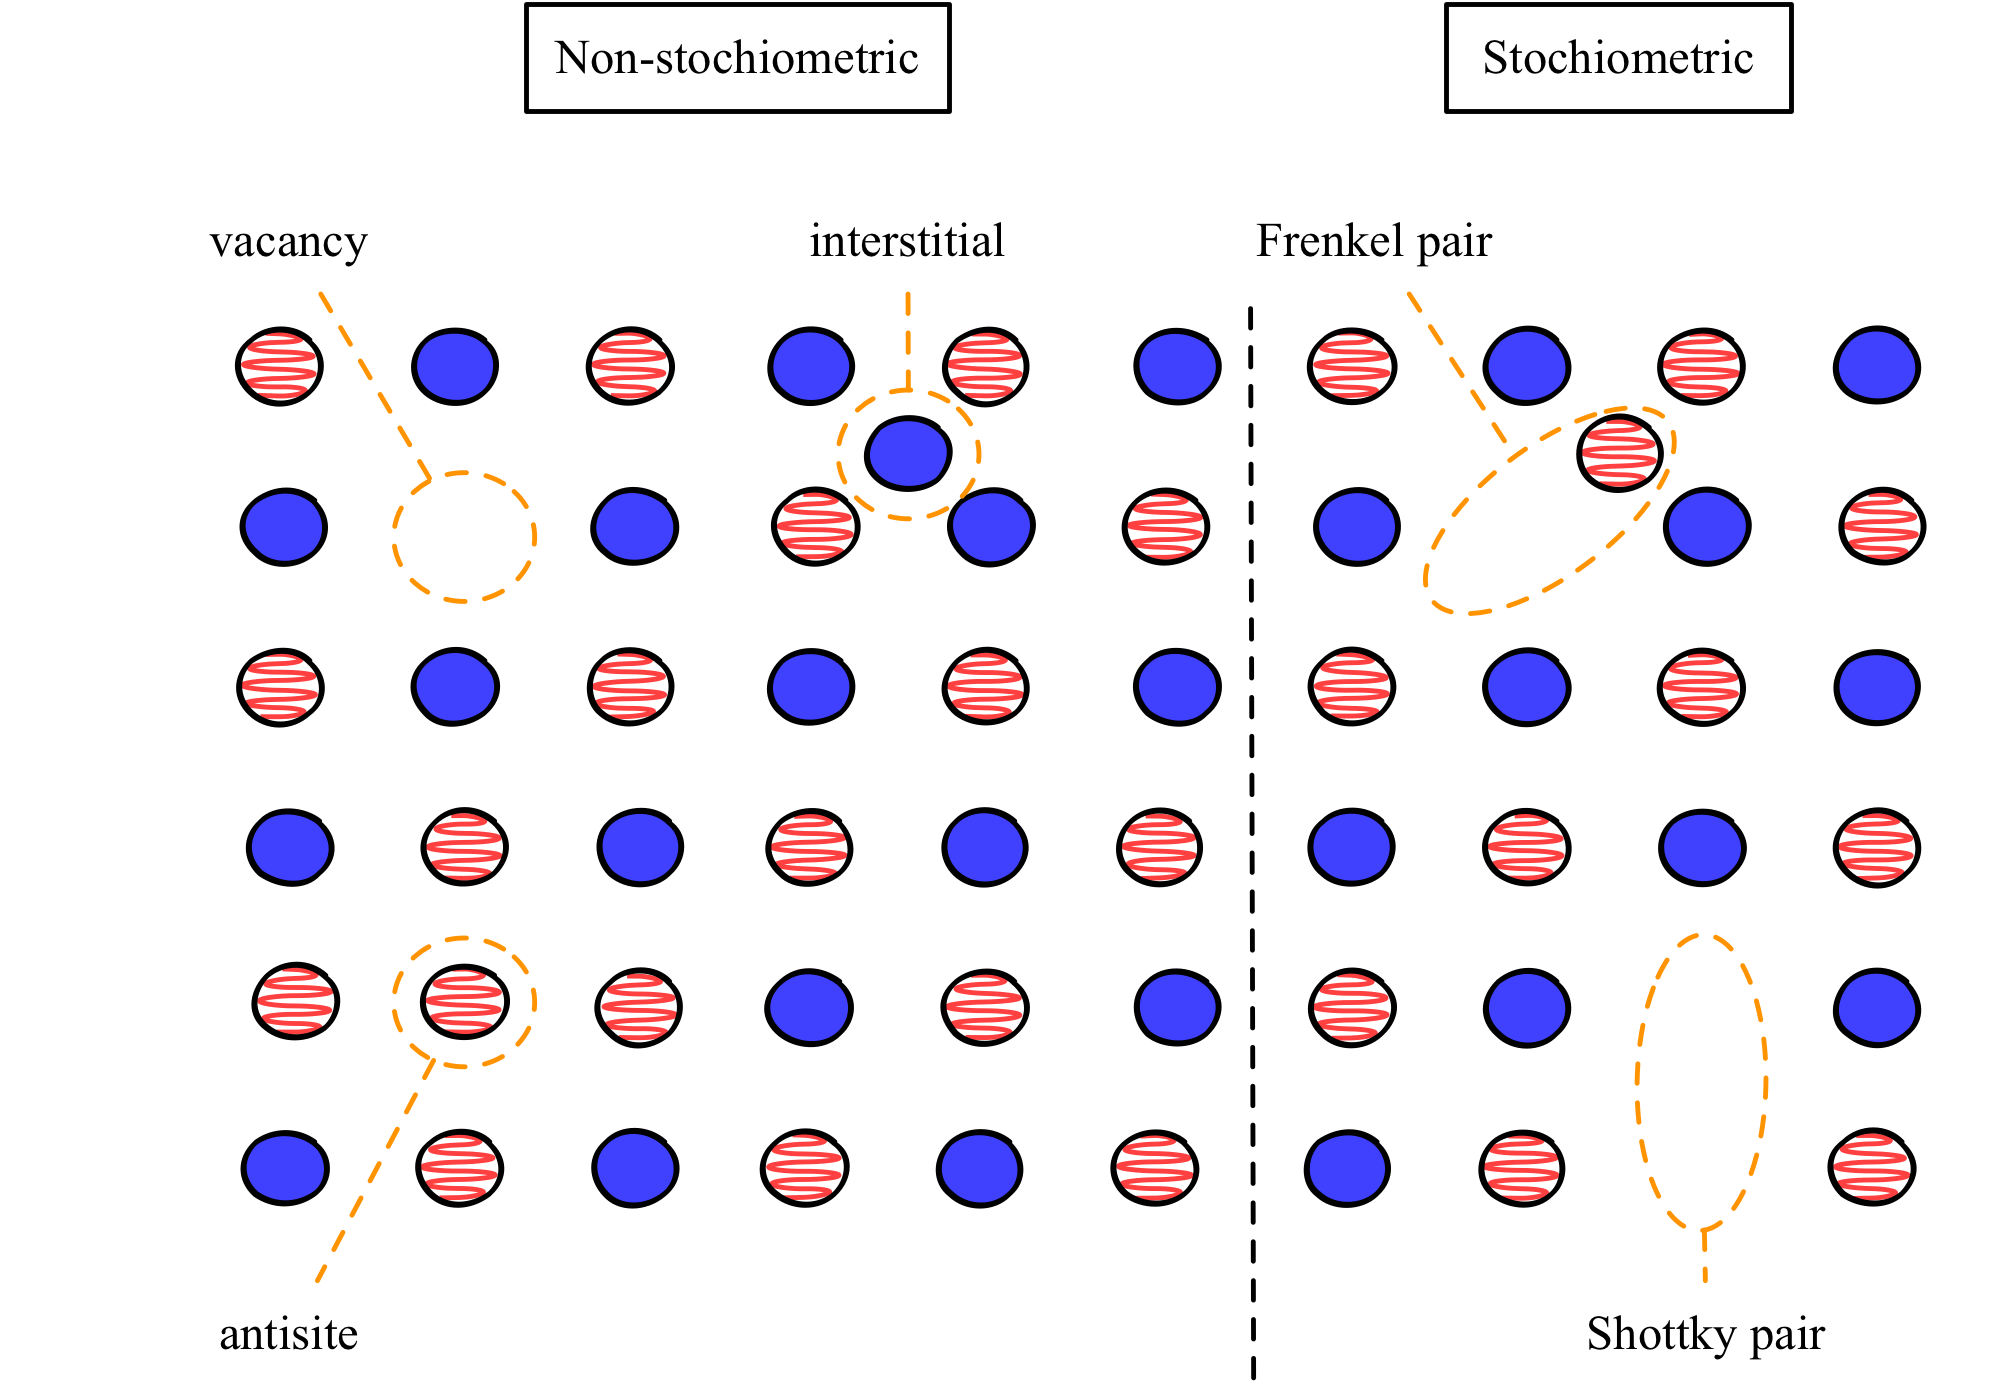
\includegraphics[width=0.8\columnwidth]{figures/ch3/classification.png}
  \caption[Classification of crystal point-defects]{Non-stochiometric defects include interstitials (an additional atom), vacancies (a missing atom) and anti-sites. Stochiometric defects include a Frenkel pair (a vacancy close to an interstitial of the same species), and a Shottky pair (a vacancy on both the anion and cation sub-lattices).}
  \label{classification} . %hatch the shapes in this drawing so can tell the differene in b+w
\end{figure}

The final classification is into electrically active and electrically benign defects. Whilst electrically benign defects exist only in one charge state, electrically active defects can take more than one charge state; for example, single acceptors exist in a neutral or negatively charged state and single donors exist in a neutral or positively charged states. Amphoteric defects can exist in a negatively charged or positively charged state.
% reference alkasukas https://www.osti.gov/pages/servlets/purl/1471061
% - may be able to say defect is there experimentally but another step to identify which it is. Admittance spectroscopy, DLTS. ESR (later chapter)
% emphasise that the concentration could be as low as one part in a milllion and wtill have an effect.
% - defect levels deend on temperature. DLTS assumes T-independent scattering cross sction, not accurate,

\subsection{Energetics of defect formation} \label{defectformation}

In the dilute limit, the equilibrium concentration of defects $n$ at a fixed temperature and pressure is given by the density that minimizes free energy.
\begin{equation} \label{defectconcentration}
    n = N_\mathrm{sites} \exp \left(-\frac{\Delta G}{k_\mathrm{B} \mathrm{T}} \right),
\end{equation}
where $\Delta G$ is the Gibbs free energy of defect formation. The Gibbs free energy is approximated as the formation energy $E_\mathrm{f}$ of the defect as this dominates over entropic contributions. The formation energy is given by:
\begin{equation} \label{eqn_formation_energy}
E_\mathrm{f}(q) = E_\mathrm{d}(q) - E_\mathrm{b} - \sum_i \mu_i n_i + q(\epsilon_\mathrm{VBM}+E_\mathrm{F}) + E_\mathrm{corr},
\end{equation}
where $E_\mathrm{d}(q)$ is the total energy of the supercell with a defect of charge $q$ and $E_\mathrm{b}$ is the total energy of the perfect bulk. 
$E_\mathrm{corr}$ is a correction energy that is needed when using a finite-sized supercell and is discussed Section \ref{corrections}.
The remaining terms describe the energy needed to add or remove atoms or electrons.
$\mu_i$ is the chemical potential of atom $i$ and can be adjusted to describe different growth conditions. 
$n_i$ is the number of atoms that are added or removed and $E_F$ is the Fermi level of the electrons, referenced to the valence band maximum $\epsilon_\mathrm{VBM}$.

The total energies can be calculated using DFT. Convergence criteria for calculations must be tight as, due to the exponential dependence of defect concentration on formation energy, small errors in the energy difference can lead to large errors in the defect concentration.

The Fermi level is treated as a parameter, of which the defect formation energy is a linear function with a gradient equal to the defect charge. This allows us to plot a graph of formation energy against Fermi level, as shown in Figure \ref{CdTeformation}. Charge transition levels mark the Fermi level at which two charge states have the same defect formation energy. Electrically active defects have at least one charge transition level in the bandgap. 
The charge transition level is equivalent to thermal ionization energy, the energy needed to add or remove electron(s). % check this
% does not always need a charge transition level deep in the bandgap. https://pubs.acs.org/doi/pdf/10.1021/acsenergylett.7b01313

\begin{figure}[h]
\centering
  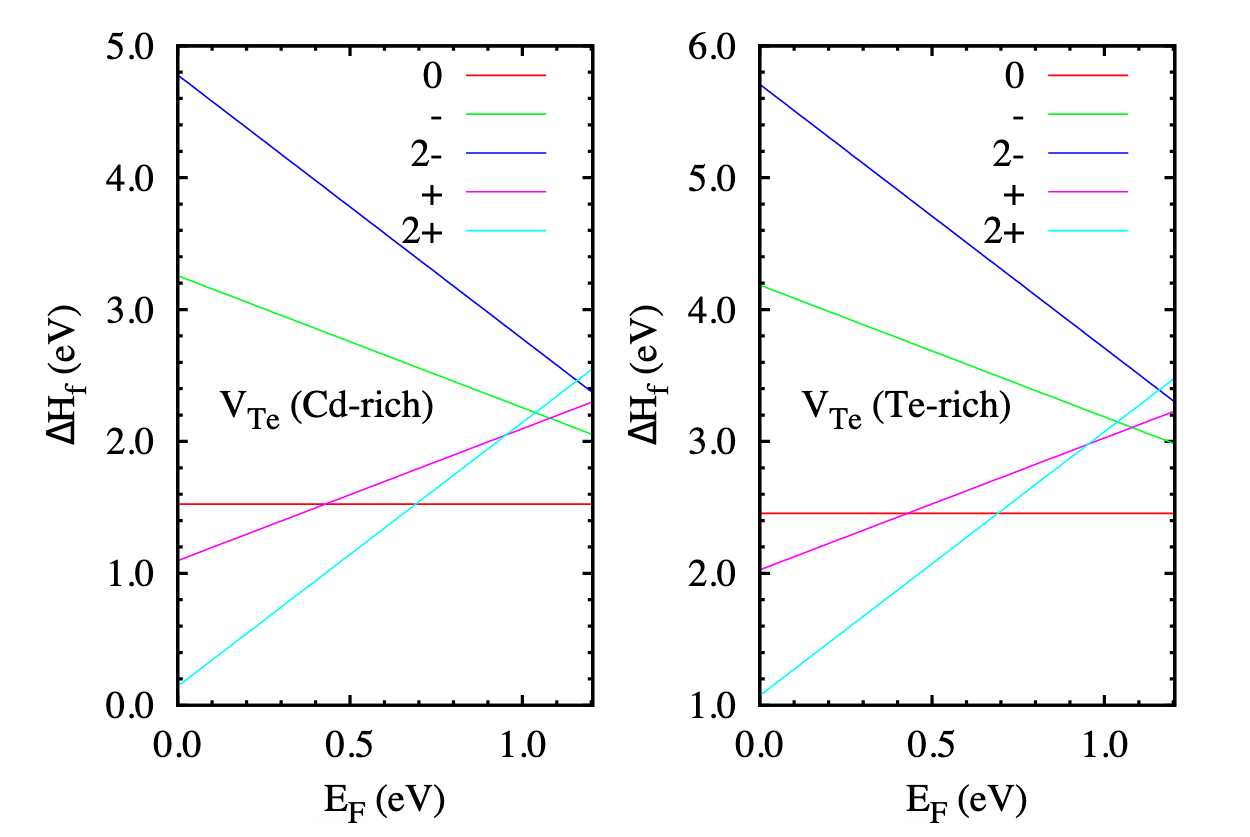
\includegraphics[width=0.8\columnwidth]{figures/ch3/defectenergetics.png}
  \caption[Formation energies of the Te vacancy in CdTe]{Formation energies $\Delta H_f$ as a function of the Fermi energy for the Te vacancy in \ce{CdTe}. In a Te-rich environment it is more energetically unfavourable to form a Te-vacancy, as intuition would suggest. The slope of each line corresponds to the defect charge. Charge transition levels correspond to the energies at which the lines intersect. Figure reproduced with permission from the work of Menendez et al.\autocite{Menendez2016}}
  \label{CdTeformation}
\end{figure}%cite https://iopscience.iop.org/article/10.1088/1742-6596/720/1/012031/pdf

Deep carrier traps have a defect level towards the middle of the bandgap and produce localised wavefunctions. Carrier capture processes to these defect states are often associated with a large lattice distortion. Shallow defect levels (within thermal energy $k_\mathrm{B}T$ of the valence or conduction band) produce delocalised, hydrogenic-like defect wavefunctions. 
% - defect energies theoretical founsations - mott littleton (1938)  - a way to calculate E the defecct energy as knew the hopping rate expression, but didnt know E. only experimental input is dielectric constant.see special 1988 issue.
%  The other problem is that is dependent upon the chemical potential which is difficult to monitor.

% Point defects result in additional energy levels in the bandgap with an associated defect wavefunction to which an electron is added or removed.
% defect level delocalised, electrical conductivity.EMT.
%or deep and localised wavefucntion. detrimental in the context of solar cells.

%The concentration of a point defect in a particular charge state can be controlled by tuning the Fermi level through doping. However there is a compensation mechanism, whereby defects form to compensate

% The concentration of point defects can be controlled by thermal treatment, irradiation or doping. 
% - Fermi level pinning (?) / defect concentration: Happens in TCO’s such as FTO. Above a certain concentration there are no more holes. This could happen when there are defect complexes which compensate each other.
% - This is a compensation mechanism. We try to adjust the fermi level of the system by introducing impurities. However above/below a certain energy level there is spontaneous formation of defects (defects which have a negative energy of formation). These defects compensate for the impurity and in this way the fermi level is pinned.

% - Calculable and observable table:
% Delta E : heat of formation / concentrations
% Defect ionisation – optical – instanataneour: PL, optical absorption / photoconductivity
% Defect ionisation , thermal, after relaxation: DLTS / thermally stimuated conductuvtiy
% Defect vibrational modes: IR/raman spectra and recombination rates

\subsection{Supercell method}

Defect concentrations as low as one part in one million can have an influence on device performance. 
One way to model point defects in the dilute limit, when defect-defect interactions are negligible, is to build a supercell from multiple unit cells (Figure \ref{translational}).
This supercell must be large enough so that there is no interaction between a defect and its periodic images.
Although the supercell method captures localised defects well, it cannot capture the behaviour of delocalised (or band resonant) defects due to the enforced periodicty. 
%http://cmt.dur.ac.uk/sjc/thesis/thesis/node71.html
To remove the constraint of translational symmetry it is possible to use an embedded QM/MM approach whereby a region around the defect is modelled using DFT and embedded in a region that is modelled classically.

% - The supercell method leads to some unphysical results for both electronic and vibrational properties. The defect will perturb the lattice. The SC method captures localised defect effects well – but the delocalised defects (possibly in the band) are not captured as there is an enforced periodicity. The only way around this is to use greens functions method (phonons) or QM/MM approach (electrons).
% vibrations of defects - link to final chapter

\subsubsection{Supercell corrections} \label{corrections}
% this is from the joint JPhysChem defects review paper - if its published I will need to cite it!
% previous section - defect-defect interaction but there are also longer ranged coloumb interations
Point defects can be electrically charged, and are able to change charge state through the trapping and de-trapping of electrons and holes. 
The charge state of a defect can affect a number of defect properties including the preferred lattice position, surrounding lattice distortion, and the rates of diffusion, carrier capture, and carrier recombination.
However, due to the long range nature of the Coulomb interaction, understanding the properties of charged defects is a challenge for DFT with periodic boundary conditions.
There are two issues to resolve: 
Firstly, charged defects can interact with their periodic images; 
Secondly, a homogeneous jellium background charge is introduced to ensure overall charge neutrality and results in an unknown shift to the average electrostatic potential. 
These are finite-size effects that only a very large, almost infinite, supercell would overcome.
However a system this size is computationally intractable, especially considering that higher levels of theory (for example, hybrid functionals) are often required to calculate accurate total energies.

A number of correction schemes have been developed to deal with these issues; a brief historical overview is given below. These schemes are designed to be used as a post-processing step and provide a value for the $E_{corr}$ term in Equation \ref{eqn_formation_energy}. A more complete description of these issues can be found in References \cite{durrant2018} and \cite{Vinichenko2017}.

The Leslie Gillan correction $E^\mathrm{LG}$ models the defect charge $q$ as a point charge interacting with its periodic images through an isotropic dielectric medium.\autocite{Leslie1985}
This correction takes a simple analytic form that depends on the charge state  $q$, static dielectric constant $\epsilon_0$, separation between defect images $L$ and the Madelung constant $\alpha_m$, which is determined by the lattice geometry:
\begin{equation}
    E^\mathrm{LG} = \frac{q^2\alpha_{m}}{2\epsilon L}.
\end{equation}
The Markov-Payne correction $E^\mathrm{MP}$ extends the Leslie Gillan correction by including an additional term that accounts for the delocalised part of the defect charge. 
\begin{equation}
    E^\mathrm{MP} = \frac{q^2\alpha_{m}}{2\epsilon L} + qQL^{-3}. 
\end{equation}
The challenge of the Markov-Payne approach is in calculating the quadrupole moment $Q$. 
The Lany-Zunger correction\autocite{Lany2009} combines the Markov-Payne correction, including an approach for calculating $Q$, with a potential alignment procedure to correct for the shift in electrostatic potential. 
The Freysholdt, Neugebauer and van de Walle (FNV) method\autocite{Freysoldt2009} models the defect charge as a localised gaussian distribution. 
The difference between the electrostatic potential of the charged defect supercell and the electrostatic potential of the perfect bulk supercell, calculated far from the defect, is aligned with the defect model potential. 
Kumagai and Oba have extended to FNV method by using atomic site potentials combined with a point charge model for an anisotropic medium.\autocite{Kumagai2014} 

There is still no standardised approach to defect charge corrections, 
which can lead to a spread in calculated defect formation energies in the literature, and predicted defect densities which differ by orders of magnitude.
Two widely used approaches in the recent literature are the FNV method, and the extension to this provided by Kumagai and Oba.
This extension is applied to the iodine interstitial defect in Chapter \ref{ch:6-defects}, using an implementation in the package \textsc{sxdefectalign}.
% - for a really good explanation see Suzys group talk (Monday the 10th september 2018) and https://aip.scitation.org/doi/10.1063/1.5029818 which it was based upon.
%what are the corections used in this work?


\section{Lattice dynamics} \label{sec:latticedynamics}
%cite defect and defect processes in nonmetallic solids
%cite Dove Lattice dynamics
This section includes a brief overview of the theory of lattice dynamics, with a particular focus on anharmonic atomic motion. The finite difference method, an intuitive way to calculate the vibrational properties of a crystal, is outlined. This method has been applied to the perfect bulk in Chapter \ref{ch:5-epcoupling} and a defect supercell in Chapter \ref{ch:6-defects}.

Heisenberg's uncertainty principle states that it is not possible to know both the position and momentum of a particle exactly. Thus the static lattice model used so far is only an approximation; even at $T=0\,\textrm{K}$ there is zero point atomic motion. As temperature increases, this vibrational motion increases in amplitude.

The lattice vibrations of a crystal must be considered to calculate a number of physical properties. Atomic motion has an associated vibrational energy, and this determines crystal stability as a function of temperature via the Gibbs free energy:\autocite{Dove1993}
\begin{equation}
G = E_0+E_\textrm{vib}+PV-TS
\end{equation}
where $E_0$ is the ground state energy, which can be calculated using DFT, and $E_\textrm{vib}$ is the vibrational contribution to internal enery.
Atomic motion also influences the electrical and optical properties of a crystal; this can be seen experimentally in the homogeneous broadening of photoluminescence linewidths with temperature, for example.\autocite{silsbee1962} %cite https://journals.aps.org/pr/abstract/10.1103/PhysRev.128.1726
Other material properties which are only accessible via lattice dynamics include: heat capacity, thermal conductivity, elasticity, thermal expansion coefficients, electron-phonon coupling strengths and static polarization.

For atomic motion at small amplitudes around the potential energy minimum it is common to use the harmonic approximation, where the atom moves as if it is connected by a spring to its neighbouring atoms (Figure \ref{harmonicregime}). This is discussed in Section \ref{harmonicapprox}. At larger vibration amplitudes, and to understand processes relating to the creation and annihilation of phonons, we must consider anharmonic motion, and this is considered in Section \ref{anharmonicapprox}.

These motions are determined by the force on each atom. For simple systems, for example a one-dimensional diatomic chain, we can calculate atomic position as a function of time analytically. Otherwise methods such as DFT can be used to build a force constant matrix which, after some post-processing steps, gives the eigenvectors (direction and amplitude) and eigenvalues (frequencies of motion). This is discussed in Section \ref{finitedisplacement}. As in the previous sections of this chapter, we use the Born-Oppenheimer approximation and assume that the equilibrium positions in a crystal are the minima of the potential energy surface when the electron and nuclear motion are decoupled.

\begin{figure}[h]
\centering
  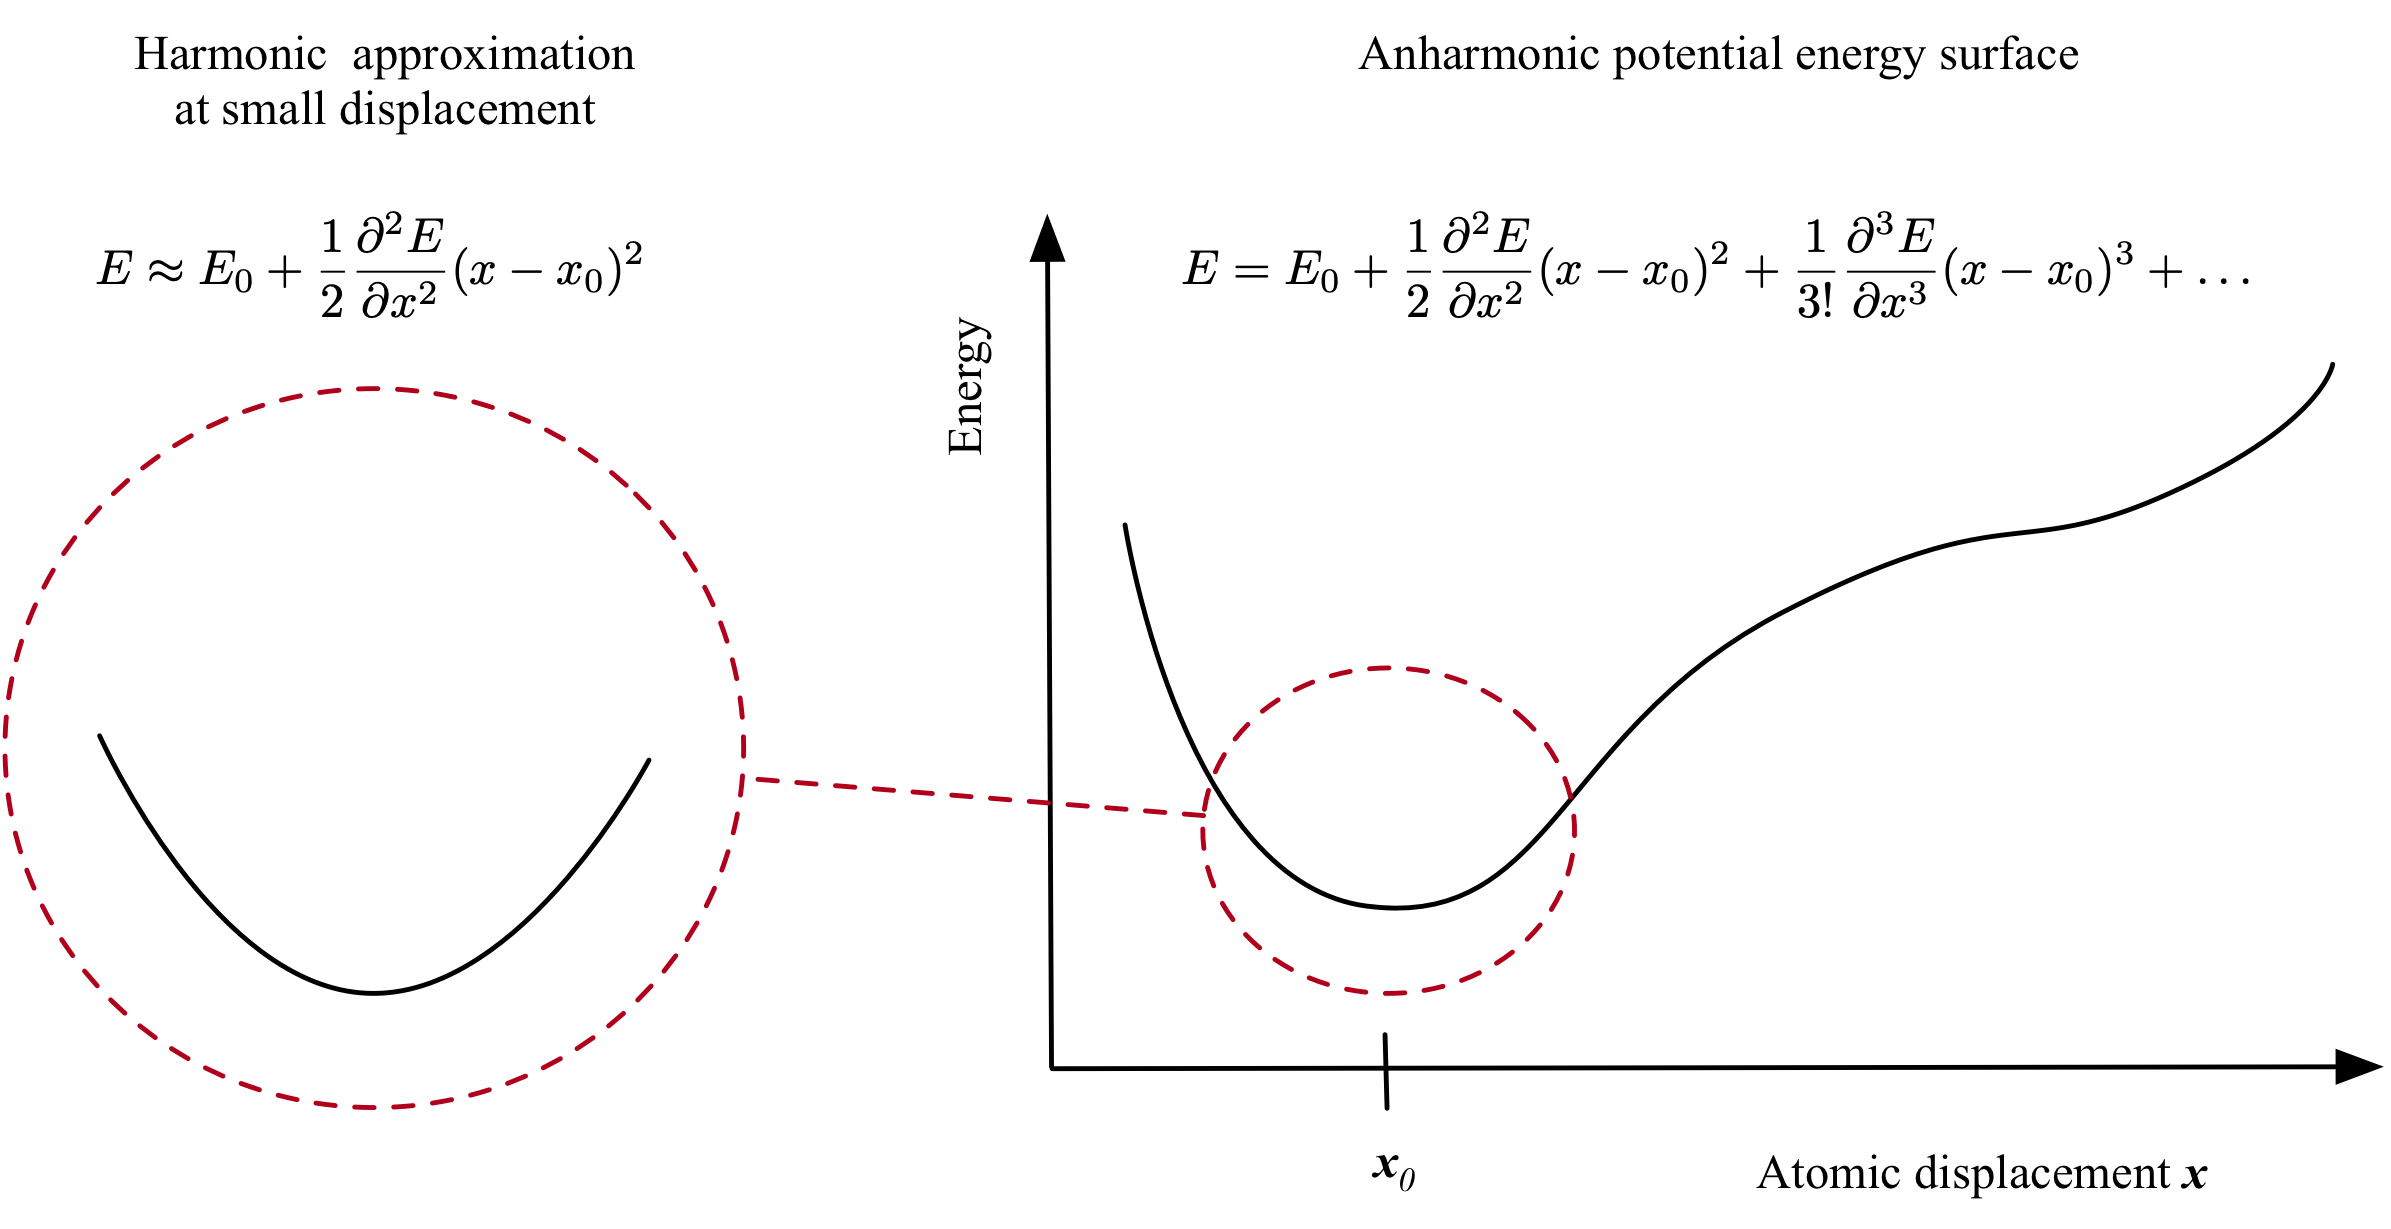
\includegraphics[width=0.8\columnwidth]{figures/ch3/harmonicregime.png}
  \caption[Crystal potential energy expanded with respect to atomic displacement]{The crystal potential energy can be expanded in powers of atomic displacement $x-x_0$, where $x_0$ is the equilibrium position. At small displacements, the anharmonic terms (third order and above) can be ignored, giving the harmonic approximation. For larger displacements, higher order anharmonic terms must be considered. The crystal lattice is relaxed so that all forces on the atoms are zero and there is no first order force term.}
  \label{harmonicregime}
\end{figure}

%important to understand crstal stabilit as the vibrational energy and entropy enter the Gibbs free energy
% - Partition function ---> bridge function kTlnZ (bridges micro and macro thermodyamics) to get helmholtz free energy. need vibrations to get temperature dependent energy and stability as a function of temperature.

% We know this affects electrical and optical properties – look at the peak shift in energy and peak broadening ith temperature.
% % - model for vibrations (harmonic approximation) ---> vib freq and displacement patterns (vibrational spectra) and from that IR/raman, free energies (T) - phase change. all stuff you couldnt get with standard electronic structure
% thermodynamics requires phonons, (helmholtz free energy)


% - What information can we get from phonons? 
% Thermodynamic quantities at low temperature: heat capacity, entropy, free energy, zero-point,
% Phase transitions from the Gibbs free energy,
% Conductivity,
% Infromation about lattice instabilities in the form of imaginary frequencies,
% Elastic tensor from the q to zero limit of phonon dispersion,
% Thermal expansion coefficient,
% Temperature dependence of the bandgap,
% Electron phonon coupling strengths,
% Static polarization

% - Experimental evidence:
% Measured directly with inelastic scattering,
% IR and Raman spectroscopy


% - For small amplitudes we consider a simple harmonic motion. phonon modes are uncoupled and have infinite lifetime.
% - At larger amplitudes we must consider anharmonic motion. phonons can be created and destroyed, have a lifetime and give access to new properties.
% - Extent of Anharmonicity depends upon how much of the potential energy space you are exploring ((tie in with perturbative and non-perturbative regime skethc). At low T you may be exploring harmonic potentil like minima, at High T you may be beyond this minima
% - Adiabatic approximation: Can thin of electronic wavefunction for eignstate of nuclei fixed in position.


% - The motions are determined by atomic forces. For a 1D system with a single mass or with two masses (lattice with basis) we can solve analytically. Otherwise these can be determined through DFT calculations (Hellman Feynmann theorem), producing a force constant matrix. 

% - Table with the approximation and the properties you can get and codes which implement....
% - quasi-harmonic:properties as a function of volume.helmholtz as function of temeparture  - at some point it is favourable to have a different volume . Free energy as function volume for several tempatures and the fit an equation of state. 
% - Then you can get the bulk modulus, heat capacity constant pressure, gibbs free, gruneisan, volumetric thermal expansion.use to get properties at finite T - use the structure which minimises for a particular temp.
% - Thermal expansion coefficients, system anharmonicity (e.g. modal grun parameters) and the temperature-dependence of other properties can be calculated in the quasi-harmonic approximation (QHA). 
% Here the lattice dynamics is harmonic at a given temperature; however, the cell volume is scaled by thermal expansion to give the first-order contribution of finite temperature effects. 
% 2: frequency and eigenvectors
% 3: phonon linewidths / spectral lifetimes
% 4: anharmonic frequency shifts
% https://thelostelectron.wordpress.com/

\subsection{Harmonic approximation} \label{harmonicapprox}

In this section I connect, using a minimum amount of mathematics, an expression for total lattice energy with the force constant matrix (which can be calculated using DFT calculations). For a more complete derivation I refer the reader to Section 2.2 of Reference \cite{Hayes1985}.

If the atomic displacement from equilibrium is small, the total energy can be Taylor expanded in the form\autocite{Hayes1985} 
\begin{align} \label{taylorexpansion}
E&=\textrm{kinetic energy}+\textrm{potential energy} \\
&=\sum_i\frac{1}{2}M\dot{x}_i^2+\sum_{ij}\frac{1}{2}\textbf{x}_i\cdot\textbf{A}_{ij}\cdot\textbf{x}_j+\textrm{higher-order terms},
\end{align}

where it is assumed that the structure is relaxed and forces are equal to zero so that there is no term linear in $\textbf{x}$. The harmonic approximation ignores the higher order terms in Equation \ref{taylorexpansion}. For these harmonic systems there exists a basis set so that $\textbf{A}_{ij}$ is diagonal and the oscillators are independent of one another:
\begin{align} \label{independentoscillators}
&=\sum_j\frac{1}{2}\tilde{M}\dot{Q}_j^2+\sum_{j}\frac{1}{2}\tilde{\textbf{A}}_{j}Q_j^2,
\end{align}
where the linear transformation has cast coordinates $x$ into $Q$.
The general solution to this system of equations for $N$-atoms in three dimensions is a superposition of $3N$ normal modes of vibration, each with its own frequency and eigenvector.
To calculate the normal modes Newton's second law, $F=ma$, is applied. For crystalline solids we take advantage of symmetry and seek normal modes $\textbf{e}(\textbf{k},t)$ that for a chosen wavevector $\textbf{k}$ are a linear combination of a relative displacement within the unit cell ($\textbf{u}_0(i,\textbf{k})$), a phase that depends on the origin $\textbf{R}_I$ of cell $I$ ($\textrm{exp}(i\textbf{k}\cdot \textbf{R}_I)$), and an oscillation in time of well defined frequency $\omega(\textbf{k})$ ($\textrm{exp}(i\omega(\textbf{k})t)$):
\begin{equation} \label{normalmodes}
\textbf{e}(\textbf{k},t) = \textbf{u}_0(i,\textbf{k})\textrm{exp}(i\textbf{k}\cdot\textbf{R}_I)\textrm{exp}(i\omega(\textbf{k})t).
\end{equation}
For displacements of this form, Newton's second law has consistent solutions only if the following secular equation is satisfied:
\begin{equation}
\textrm{Det}||\sum_J A_{\alpha\beta}(iI,jJ)\textrm{exp}(i\textbf{k}\cdot\textbf{R}_J)-M_i\delta_{ij}\omega^2(\textbf{k})||=0,
\end{equation}
where the first term in the determinent is the dynamical matrix. The dynamical matrix is built from the force constant matrix $A_{\alpha\beta}$:
\begin{equation} \label{forceconstant}
\textbf{A} = 
\begin{pmatrix} 
\frac{\partial^2E}{\partial x_1^2} &\frac{\partial^2E}{\partial x_1 \partial x_2} & \cdots & \frac{\partial^2E}{\partial x_1 \partial x_n}\\
\frac{\partial^2E}{\partial x_2 \partial x_1}&\frac{\partial^2E}{\partial x_2^2} & \cdots & \frac{\partial^2E}{\partial x_2 \partial x_n}\\
\vdots & \vdots & \ddots & \vdots \\
\frac{\partial^2E}{\partial x_n \partial x_1}&\frac{\partial^2E}{\partial x_n \partial x_2} & \cdots & \frac{\partial^2E}{\partial x_n^2}\\
\end{pmatrix}
\end{equation}

The normal mode frequencies $\omega(\textbf{k})$ are roots of the secular equation \ref{normalmodes} and can be found through matrix diagonalisation. Plotting the frequency $\omega$ against wavevector $\textbf{k}$ for a lattice with a periodicity of length $L$ gives a bandstructure plot with a periodicity of $\frac{2\pi}{L}$.   %check that a is correct for lattice length 

The discussion so far has only used classical mechanics. To introduce quantum effects we recognise that the harmonic lattice vibrations are analogous to a quantum simple harmonic oscillator and so will be restricted to certain energy values $E_n = \hbar\omega(\textbf{k})(n+\frac{1}{2})$.
The discrete (quantised) unit of energy $\hbar\omega(\textbf{k})$ is a phonon quasiparticle that corresponds to a collective excitation of the crystal lattice.
% The phonons of energy hbar omega have exact energy so cannot be localised in space: formed of delocalised plane waves
% But can construct localized packet using modes of different fequency. Can then treat phonons as localised particles. E = hbar omega. K is the crystal momentum .
% Phonons are bosons, not conserved. They can be created and destroyed. 
% once got eigencevtors nad freuencies have access to toher props via partition function

\subsection{Anharmonicity} \label{anharmonicapprox}

Anharmonic atomic motion is described by the higher order terms in Equation \ref{taylorexpansion}.
The third order term accounts for phonon-phonon scattering which, due to the conservation of energy and momentum, is a three particle process (Figure \ref{anharmonicity}).\autocite{Lundstrom2000}

The linear boltzmann transport equation (LBTE) describes a thermodynamic system out of equilibrium. Solving the LBTE under the single mode relaxation time approximation gives an expression for the lattice thermal conductivity $\kappa$.
The phonon-phonon scattering rate determines the phonon lifetime $\tau_\lambda$ which is a key quantity in the expression for $\kappa$:\autocite{Togo2015a}
\begin{equation}
    \label{thermalconductivity}
    \kappa=\frac{1}{NV_0}\sum_\lambda C_\lambda v_\lambda \times v_\lambda \tau_\lambda,
\end{equation}
where $N$ is the number of unit cells in the crystal, $V_0$ is the unit cell volume, and $C_\lambda$, $v_\lambda$ and $\tau_\lambda$ are the mode-dependent heat capacity, group velocity and lifetime respectively. $C_\lambda$ and $v_\lambda$ can be calculated using the harmonic approximation. To quantify the strength of the anharmonic phonon interactions that determine $\tau_\lambda$ it is necessary to calculate a third-order force constant matrix. This is often at high computational cost; in Reference \cite{Whalley2016} 41,544 DFT calculations were required to calculate the thermal conductivity of a 96-atom unit cell.
% -  can reduce the cst by just considering the phase space (broido talk, laptop notes)

Lattice anharmonicity can also be used to describe materials with dynamic disorder. In the halide and oxide perovskites the onset temperature for dynamic disorder is determined by the depth of the double well potential energy surface (Figure \ref{thermalconductivity}).\autocite{Yang2017}
Chapter \ref{ch:5-epcoupling} calculates the coupling between the anharmonic double well phonon modes and electronic states in MAPI.
 % - anharmonicity schematic under visuals: Si, PbTe, SrTiO3% - Anharmonicity also needs to be considered according to material (schematic here)
% for some vobrations compression and extension will not be equal curvature. talk about % - harmonic approximation expects the energy to increase as you push along the mode.imaginary frequency because $w^2$ is negative.
% - dynamic stability if all positive
%- mechanism for some phase transitions is where phonon mode becomes imaginary at a transition temperature
% frozen phonon approximation


% - Anharmonicity most important when under high pressure or high temperature (bouchert) which is often the case for geophysical applications.
% - Navaneeth : assessing how higher order anharmonicity can aggect htermal conductivity. In Diamond the 4 phonon phase space is 10x that of 3-phonon. In Bas it is 100X that of 3-phonon phase space. We must then also consider the scattering strength (can only consider the scattering rate of those with a large phase space). The size of these phase spaces are huge. For example, Bas which is in the zincbelnde structure has 6 polarisations. If each done explicitly there would be $9x10^ 3$-phonon calculations, for 4-phonon processes there would be $2x10^12$!!!  So instead temperature-dependent ensembles are used (where all atoms are moved at the same time, calculated from explicit 2nd order force constant calculation) and then used to fit 3rd and 4th order force constants to.



\begin{figure}[h]
\centering
  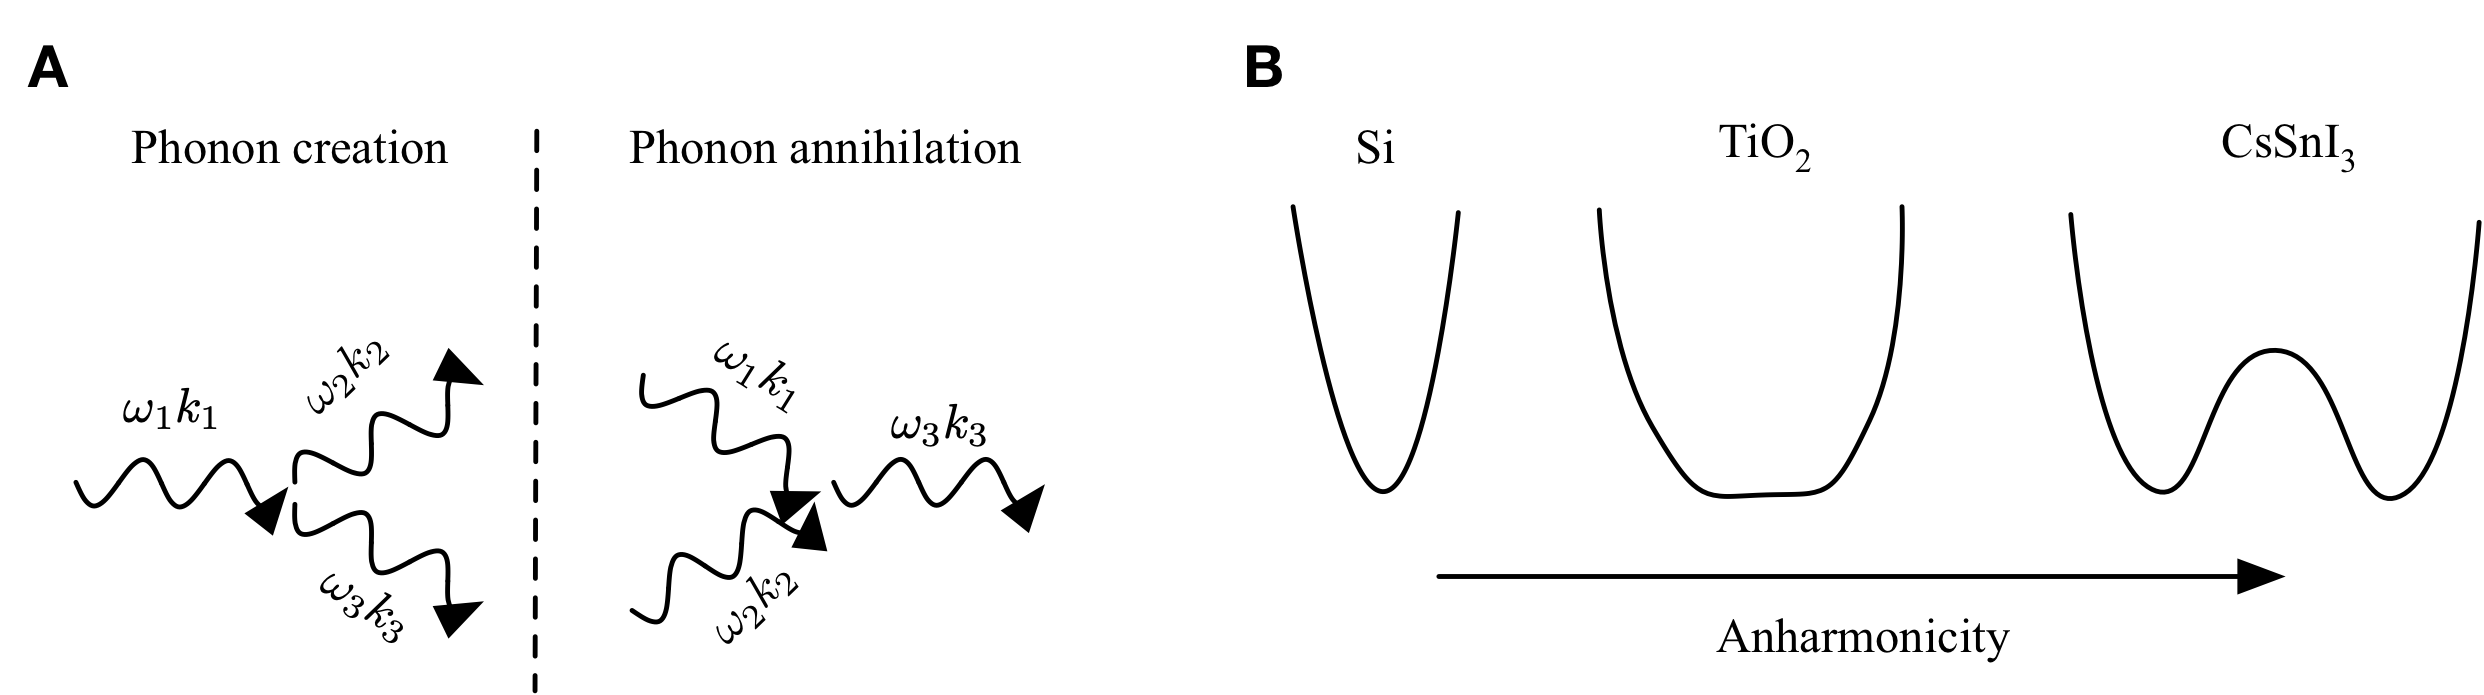
\includegraphics[width=1.0\columnwidth]{figures/ch3/anharmonicity.png}
  \caption[3-phonon processes and anharmonic potential energy surfaces]{A) Energy and momentum are conserved during the creation or annihilation of phonons, so these are three-phonon processes (or higher); B) Some materials, such as silicon (Si) are well-described by a harmonic potential energy surface at typical solar cell operating temperatures. However other materials with dynamic disorder, such as the organic and inorganic perovskite halides, have highly anharmonic double well potentials.}
  \label{anharmonicity}
\end{figure}  %include phonon-phonon scattering schematic? the third regime where important is given in the other figure, at high temperature %cite ruoxi work



\subsection{Finite displacement method} \label{finitedisplacement}

There are a number of ways to calculate the second order force constant matrix in Equation \ref{forceconstant} including: the finite displacement method; density functional perturbation theory; ab-initio molecular dynamics and compressed sensing lattice dynamics.
In this work the finite displacement method (also known as the direct or supercell method) is used: a single atom is displaced a small distance from its energetic minimum and there is a self-consistent electronic structure optimisation to calculate the resultant forces. The maximum number of displacements for a system with $N$ atoms in the unit cell is $6N$, although this is reduced through symmetry. 
To consider phonon wavelengths greater than the unit cell length a supercell is required, and all forces must be well converged (typically to less than \SI{0.01}{\electronvolt\per\angstrom}).

%negatives of this approach: no long range forces beyond hte supercell (polar materials), no anharmonicity .  %positive - highly parallelisable

% - Note that the  eigenvalue equation for the dynamical matrix is gotten from fourier transform
% Of the taylor expansion of the crystal potential.
% - force constant matrix . then construct dynamical matrix - -> wavevector. then diagonalise - the eigenvectors and eigenvalues. do a schematic for this process. then two ways to get to the dynamical matrix.

% - There are a multitude of ways to calculate these force constants: explicitly (finite difference, DFPT for 3rd or 4th orders), empirical potentials (TDEP), compressive sensing lattice dynamics or beyond perturbation (AIMD,PIMD,SCAILD, variational methodslike SSCHA developed by Ion Errea).
% - perturbation theory- dynamical matrix directly. no supercell and more accurate but constrained which functionals and pseudopotentials you need.

% schematic of workflow: input structure, create displacements, calculate forces, calculate dynamical matrix, diagonalise

% phonon workflow

% in this work the finite displacement approach is used as implemented in...
% For derivatives we exploit the hellman-feynam theorem and use finite differences % - Force constant via finite displacement - displace small and calculate force. Simple, general and can split into small jobs (parallelise). 
% AKA "supercell","direct" or "frozen phonon" 
% - phonons can have a wavelength longer than the size of the supercell - need to capture the longer wavelength. but need supercells. use phonopy. Maximum is 6N displacements but this is seriously reduced by symmetry. (spglib)
% - Need good relaxation: don't skimp on the forces, cutoff or k-points.
% - PBEsol for reproducing lattice constants and phonons (Jonathan 2015 J.Chem. Phys)

% - See Jonathans talks

\section{Summary}

In this chapter I have introduced the key concepts that underly DFT, and the post-processing steps required to calculate the defect and vibrational properties of a crystal. 
Much of solid state physics is built upon the idea of a translationally invariant crystal, so it should come as little surprise that additional steps are needed to describe defects that break translational symetry and work against the fundamental assumptions of the theoretical framework.
In contrast, phonons at the gamma point preserve the underlying translational symmetry, but additional steps are needed to build the force constant matrix from multiple DFT calculations.
In this chapter I have presented the defect and vibrational calculations separately. In Chapter \ref{ch:6-defects} I combine the two approaches, and calculate the vibrational properties of the iodine interstitial defect in MAPI. 
%A discussion about how a point defect perturbs the vibrational sub-system of a bulk material is included in that final chapter.
%: LW - could we add here that solid state physics of crystalline materials is not really built for defects as they assume perfect translational symmetry, which the defects break ---> which makes modelling defects a continuing challenge for theory and simulation (as we are working "against" the fundamental assumptions of the framework).
% - defects are demainding and computational expensive .n To avoid computationally expensive defect calculations descriptors have been built on the idea of ‘defect tolerant’ materials: http://pubs.acs.org/doi/pdf/10.1021/acs.nanolett.5b04513
% in fact I combine defect and phonon calculations in final chapter


